\documentclass[a4paper,12pt,oneside,openany]{book}%book o scrbook, da provare; twoside per libro; b5 per libro piccolo
\usepackage[T1]{fontenc}
\usepackage[utf8]{inputenc}
\usepackage[italian]{babel}
%\usepackage{layaureo}
\usepackage[eulerchapternumbers,beramono,pdfspacing]{classicthesis}
\usepackage{arsclassica}
\usepackage{graphicx}

\begin{document}
	\author{Sandro Della Maggiore}
	\title{\Huge HEGEL\\{\Large e l'idealismo logico}}
	\date{Marzo 2024}
	\maketitle

\section*{I CAPISALDI DEL SISTEMA HEGELIANO}
	
Per poter comprendere il pensiero di Hegel risulta indispensabile aver chiare, sin dall’inizio, le tesi di fondo del suo idealismo:

\begin{enumerate}
	\item  la risoluzione del finito nell’infinito;
	\item l’identità fra ragione e realtà;
	\item la funzione giustificatrice della filosofia.
\end{enumerate}

\subsection*{Finito e infinito}

Con questa espressione, Hegel intende dire che la realtà non è un insieme di sostanze autonome, ma un organismo unitario, detto Assoluto, di cui tutto ciò che esiste è parte o manifestazione. Tale organismo, non avendo nulla al di fuori di sé e rappresentando la ragion d’essere di ogni realtà, coincide con l’Infinito. Lungi dall’essere una totalità armoniosa, l’Assoluto hegeliano si presenta come una totalità articolata che unisce parti, i vari enti del mondo, detti finiti, che sono diverse e anche opposte tra loro, senza annullarne le differenze. L’Assoluto risulta essere quindi l’UNIONE DELL’UNIONE E DELLA NON UNIONE, “sintesi di identità e differenza“. Nell’Assoluto, la conflittualità non lacera l’unità ma la rende più ricca, divenendo la condizione che ne favorisce la realizzazione. I finiti, essendo manifestazioni di esso, coincidono con l’infinito. Pertanto, il finito, come tale, non esiste: ciò che noi chiamiamo “finito” è nient’altro che un’espressione parziale dell’Infinito. Infatti, come la parte non può esistere se non in connessione con il Tutto, in rapporto al quale soltanto ha vita e senso, così il finito esiste unicamente nell’infinito e in virtù dell’infinito. Detto altrimenti: il finito, in quanto è reale, non è tale, ma è lo stesso infinito.

Se la concezione cristiana si basa sulla fede in un Dio creatore trascendente e ontologicamente distinto dal creato, l’hegelismo si configura come una forma di monismo panteistico: esiste un’unica realtà divina (monismo) di cui il mondo visibile costituisce la realizzazione o la manifestazione.  Tuttavia il panteismo di Hegel si differenzia da quello moderno di Giordano Bruno e di Spinoza: per entrambi  l’Assoluto è una Sostanza statica che coincide con la Natura ma incapace di spiegare cosa la spinga a differenziarsi in molti concetti e a presentarsi in infinite forme particolari; per Hegel invece l’Assoluto si identifica con un Soggetto spirituale in divenire, come una realtà spirituale che ha il carattere della trasformazione, del continuo “farsi altro”, di cui tutto ciò che esiste è un “momento” o una “tappa” di realizzazione. La totalità è movimento, processo, divenire, trasformazione: è – dice Hegel – vita. Le differenze e le opposizioni, come già detto, non si annullano, bensì interagiscono in un processo continuo, in un farsi infinito. Infatti, dire che la realtà non è “Sostanza”, ma “Soggetto”, significa dire, secondo Hegel, che essa non è qualcosa di immutabile e di già dato, ma un processo di auto‑produzione che soltanto alla fine, cioè con l’uomo (= lo Spirito, che è piena “consapevolezza della totalità”), giunge a rivelarsi per quello che è veramente: “Il vero ‑ scrive Hegel nella Prefazione alla Fenomenologia dello Spirito ‑ è l’intero. Ma l’intero è soltanto l’essenza che si completa mediante il suo sviluppo. Dell’Assoluto devesi dire che esso è essenzialmente Risultato, che solo alla fine è ciò che è in verità…”. In altre parole, poiché la totalità è processo, la verità è il culmine del processo. Il divenire dello Spirito comprende inevitabilmente momenti drammatici di conflitto, di lacerazione, di sconfitta, in altre parole, di negazioni e differenze, ricondotte ad un’unità superiore, come vedremo, dalla ragione. La filosofia, scrive Hegel, deve attraversare il suo “venerdì santo speculativo” prima di arrivare alla domenica di Pasqua. Ma proprio qui sta la novità di Hegel: il negativo non è l’ultima parola. Il negativo è un momento essenziale del positivo e dell’Assoluto concreto verso cui si tende. Il movimento stesso è reso possibile dalle differenze, o “opposizioni”, e dal superamento in un’unità superiore, che genera altre opposizioni e altre unificazioni, e così via. Il pensiero, dunque, è un processo in cui i concetti trapassano l’uno nell’altro, attraverso opposizioni e sintesi continue.

\subsection*{ Ragione e realtà}

Il Soggetto spirituale infinito che sta alla base della realtà viene denominato da Hegel con il termine di Idea o di Ragione. E’ proprio l’idea, cioè il pensiero, a permetterci di scoprire nei fenomeni che ci circondano costanti, regolarità, leggi. Tali leggi non esistono soltanto nella nostra mente ma anche nella realtà. Hegel riabilita l’idea greca del logos: il logos è sia l’ordine razionale della realtà, sia il ragionamento, sia il discorso umano sulla realtà.  In questo modo Hegel sostiene l’identità di pensiero ed essere, o meglio, di ragione e realtà, vale a dire dell’unità originaria. Per Hegel è quindi inammissibile il dualismo di pensiero e realtà come sostanze separate ed eterogenee. Il pensiero è realtà e la realtà è pensiero, spirito. Ciò implica anche che tra logica ed ontologia (o metafisica) non sussiste alcuna differenza. Da ciò il noto aforisma, contenuto nella Prefazione ai Lineamenti di filosofia del diritto, che è stato oggetto delle più svariate interpretazioni, in cui si riassume il senso stesso dell’hegelismo: Ciò che è razionale è reale; e ciò che è reale è razionale.

Con la prima parte della formula, Hegel intende dire che la razionalità non è pura idealità, costruzione astratta, schema, dover‑essere, ma la forma stessa di ciò che esiste, poiché la ragione “governa” il mondo e lo costituisce. In altre parole, se l’Assoluto non si incarna nel mondo è vuoto, astratto, formale.

Con la seconda parte della formula, Hegel intende affermare che la realtà è una connessione unitaria che ha i caratteri della necessità, cioè non è un confuso insieme di avvenimenti casuali, non è una materia caotica, ma il dispie­garsi di una struttura razionale (l’Idea o la Ragione) che si manifesta in modo inconsapevole nella natura e in modo consapevole nell’uomo: se il reale non si riconosce nel razionale è privo di significato, è senza senso. Per cui, con il suo aforisma, Hegel non esprime la semplice possibilità che la realtà sia penetrata o intesa dalla ragione, ma la necessaria, totale e sostanziale identità di realtà e ragione. Tuttavia tale identità non va intesa semplicemente e staticamente: essa implica anche l’identità fra essere e dover‑essere, in quanto ciò che è risulta anche ciò che razionalmente deve essere. Tant’è vero che le opere di Hegel sono costellate di osservazioni piene di ironia e di scherno a proposito dell’“astratto” e moralistico dover essere che non è, dell’ideale che non è reale. Il mondo, in quanto è e così com’è, è razionalità dispiegata, ovvero ragione reale e realtà razionale che si manifesta attraverso una serie di momenti necessari che non possono essere diversi da come sono. Infatti, da qualsiasi punto di vista guardiamo il mondo, troviamo ovunque, secondo Hegel, una rete di connessioni necessarie e di “passaggi obbligati” che costi­tuiscono l’articolazione vivente dell’unica Idea o Ragione. In altri termini, Hegel, secondo uno schema tipico della filosofia romantica, ritiene che la realtà costituisca una totalità processuale necessaria, formata da una serie ascendente di “gradi” o “momenti”, che rappresentano, ognuno, il risultato di quelli precedenti ed il presupposto di quelli seguenti.

\subsection*{La funzione giustificatrice della filosofia}

Coerentemente con il taleorizzonte teorico, fondato sulle categorie di totalità e di necessità, Hegel ritiene che il compito della filosofia consista nel prendere atto della realtà e nel comprendere le strutture razionali che la costituiscono: “Comprendere ciò che è è il compito della filosofia, poiché ciò che è è la ragione”. Compito della filosofia non è quella di dare delle lezioni di razionalità al reale perché il reale è già razionale: a dire come dev’essere il mondo, la filosofia arriva sempre troppo tardi giacché sopraggiunge quando la realtà ha compiuto il suo processo di formazione. Essa, afferma Hegel con un paragone famoso, è come la nottola di Minerva, la civetta che accompagna la dea della sapienza, che inizia il suo volo sul far del cre­puscolo, cioè quando la realtà è già bell’e fatta. La civetta, infatti, ha grandi occhi ed è capace di vedere nella notte. Così la filosofia, in una buia epoca di crisi e di passaggio tra il vecchio e il nuovo, ha la capacità di vedere i fenomeni. La filosofia deve dunque “mantener­si in pace con la realtà” e rinunciare alla pretesa assurda di determinarla e guidarla. Deve soltanto portare nella forma del pensiero, cioè elaborare in concetti, il conte­nuto reale che l’esperienza le offre, dimostrandone, con la riflessione, l’intrinseca razionalità e necessità. Si è sempre visto in essa il simbolo stesso della vocazione contemplativa e della rinuncia alla trasformazione del mondo da parte di Hegel: sembra, infatti, che egli affidi al pensiero il compito di registrare passivamente una situazione storica già svoltasi e di rifugiarsi nella notte della propria interiorità. La filosofia, infatti, non può fornire programmi d’azione politica perchè esprimono consapevolezze che possono maturare solo dopo che un’epoca si è conclusa.
In Hegel troviamo un altro animale simbolo in contrappeso alla civetta: la talpa. La talpa, presente nelle berlinesi Lezioni sulla filosofia della storia, costruisce percorsi complessi e ordinati attraverso un lavora sottoterra, uno scavo incessante nel buio più totale, guidata soltanto dall’istinto di un senso dello spazio particolarmente sviluppato. In Hegel, simbolizza il cammino della storia come un progressivo affermarsi della razionalità inconscia contenuta implicitamente nell’attività degli uomini, nella costruzione di un mondo storico. Al contrario, la civetta è capace di vedere nel buio ma non di agire. Il contributo della filosofia consiste (al pari dell’intervento dello Stato nella sfera economica della società civile) nel chiarire e mitigare i conflitti. È un’immagine che proviene dall’Amleto di Shakespeare, un autore che ha avuto un peso enorme in Hegel, molto più di tanti filosofi, grazie alla sua visione tragica, e anche “dialettica”, della storia. Quindi mentre la filosofia contempla, la storia lavora. In Hegel queste due immagini hanno un equivalente nei popoli: i tedeschi sono la civetta, sono un popolo contemplativo; i francesi, per converso, agiscono molto, ma magari pensano poco. Per cui Hegel, come il giovane Marx, che fonderà una rivista chiamata Annali franco-tedeschi, è in favore di questa unione virtuosa tra l’intellighenzia tedesca e la capacità politica e trasformatrice dei francesi. In realtà, Hegel esalta il campo d’azione della filosofia, come si legge in una lettere del 1808: “Il lavoro teoretico, me ne vado convincendo ogni giorno di più, produce nel mondo più che non il pratico; una volta rivoluzionato il regno della rappresentazione, la realtà effettuale non tiene più“. Questi chiarimenti delineano il tratto essenziale della filosofia e della personalità di Hegel. L’autentico compito che Hegel ha inteso attribuire alla filosofia (e ha cercato di realizzare con la sua filosofia) è la giustificazione razionale della realtà, della presenzialità, del fatto.

Hegel in un passo dell’Enciclopedia ha precisato che la sua filosofia non può essere scambiata per una banale accettazione della realtà in tutti i suoi aspetti, perché non vanno inclusi nel concetto di “realtà” gli aspetti superficiali e accidentali dell’esistenza. Per Hegel è “razionale” e dunque “reale” ciò che nella storia avanza, producendo effetti, non ciò che nella storia viene colto istantaneamente. Tuttava come possa esistere l’accidentale in una realtà razionale e necessaria resta oscuro. Gli “accidenti” rappresentano ciò che non si lascia ridurre alla ragione, cioè alla sua filosofia.

Nella vita ordinaria si chiama a casaccio realtà ogni capriccio, l’errore, il male e ciò che è su questa linea, come pure ogni qualsiasi difettiva e passeggera esistenza. Ma già anche per l’ordinario modo di pensare un’esistenza accidentale non meriterà l’enfatico nome di reale: l’accidentale è un’esistenza che non ha altro maggior valore di un possibile, che può non essere allo stesso modo che é. Ma, quando io ho parlato di realtà, si sarebbe pur dovuto pensare al senso nel quale adopero quest’espressione, giacché in una mia estesa Logica ho trattato anche della realtà, e l’ho accuratamente distinta non solo dall’accidentale, che pure ha esistenza, ma altresì dall’essere determinato, dall’esistenza e da altri concetti.

Questo compito egli l’ha affrontato con maggiore energia proprio là dove esso sembra più rischioso: cioè nei confronti della realtà politica, dello Stato: infatti può sembrare ovvio che il mondo naturale sia razionale, in quanto regolato da leggi necessarie, mentre è più difficile riconoscere che qualsiasi costruzione storica dell’uomo sia l’espressione di una necessità razionale, e che quindi debba essere accettata così com’è.

A partire da questa precisazione taluni critici hanno negato il carattere giustificazionista della filosofia hegeliana: un filone interpretativo che va da Engels a Marcuse (pensatori della “sinistra rivoluzionaria”), pur ammettendo gli aspetti conservatori del pensiero hegeliano, ha tuttavia cercato di mostrare come esso possa venir letto in modo dinamico e rivoluzionario. Infatti, secondo tali autori l’aforisma di Hegel significherebbe in sostanza che il reale è destinato a coincidere con il razionale, mentre l’irrazionale è destinato a perire. In altre parole, non tutto ciò che è semplicemente esistente è reale, ma ciò che ha la potenzialità di trasformarsi. Ora, questa lettura di Hegel rappresenta, più che un’interpretazione, una correzione di Hegel alla luce degli ideali rivoluzionari dei suoi autori. In conclusione ci sembra che i testi di Hegel documentino in modo chiaro e inequivocabile il suo atteggiamento fondamentalmente giustificazionista nei confronti della realtà.

\newpage
	
	\section*{Idea, Natura e Spirito. La partizione della filosofia.}
	
Il disegno complessivo dell’Enciclopedia hegeliana è quello di una grande triade dialettica in cui l’Assoluto, cioè la ragione, nella sua verità, deve giungere a riconoscersi come reale e ciò compare solo alla fine del processo, quale risultato conclusivo. Ciò non significa che l’Assoluto non sia compiuto già all’inizio, ma la verità è tale solo se confermata dalla totalità dello sviluppo. Il reale è già razionale e la ragione è già reale, solo che essa non ne è pienamente consapevole. Per giungere a questa consapevolezza deve percorrere un itinerario, un processo per l’appunto, che è tutt’altro che scevro di difficoltà: per riconoscersi nel reale, la ragione deve scontrarsi innanzi tutto con ciò che non si lascia ridurre ad essa, con qualcosa che la nega. Si tratta della già nota dialettica idealistica, presente anche in Fichte e Schelling, tra limite e superamento di esso da parte dello spirito che riconduce ogni realtà all’identità con sé.

Quindi, anche Hegel ritiene che il farsi dinamico dell’Assoluto passi attraverso tre momenti: l’Idea in sé (tesi), l’Idea fuori di sé (antitesi) e l’Idea in sé e per sé, che ritorna in sé (sintesi). Solo realizzando il ricongiungimento del primo e dell’ultimo momento, l’Assoluto giunge al proprio maturo compimento, mostrandosi come soggetto autoconsapevole delle proprie forme e delle proprie manifestazioni. La verità deve dunque superare la prova del fuoco della realtà. La dialettica è il percorso che l’Assoluto compie per giungere alla sua verità; è il percorso attraverso cui l’Assoluto, inizialmente inconsapevole e puro essere in sé, si appropria delle sue stesse manifestazioni, che prima esperisce come qualcosa di estraneo, come un essere fuori di sé, acquisendo quell’autoconsapevolezza che Hegel esprime attraverso la nozione riflessiva di essere per sé.

Nella fase matura del pensiero hegeliano questo schema dialettico generale articolerà i contenuti di un sistema completo di filosofia, secondo tre momenti principali: logica (tesi), natura (antitesi) e spirito (sintesi). A questi tre momenti strutturali dell’Assoluto Hegel fa corrispondere le tre sezioni in cui si divide il sapere filosofico:

\begin{figure}[h]
	\centering
	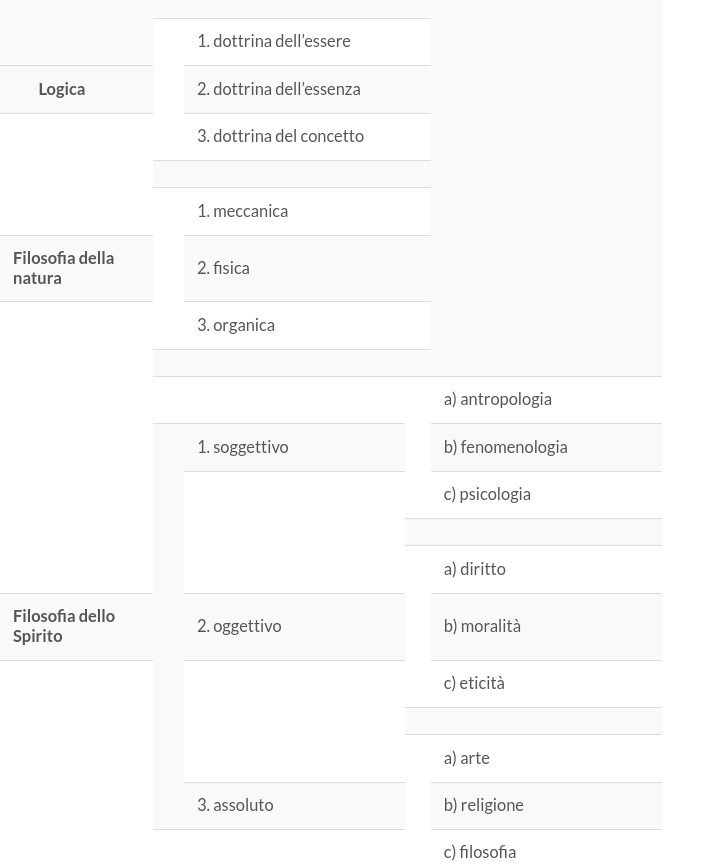
\includegraphics[width=0.8\linewidth]{Filosofia_Hegel}
	\caption[Schema filosofia Hegel]{}
	\label{fig:filosofiahegel}
\end{figure}



\begin{enumerate}
	\item La logica, che è la scienza dell’Idea in sé, cioè dell’Idea “pura”, considerata in se stessa (= in sé) a prescindere dalla sua concreta realizzazione nella natura. Da questo angolo prospettico, l’Idea, secondo un noto paragone teologico di Hegel, è assimilabile a Dio prima della creazione della natura e di uno spirito finito, ovvero, in termini meno equivocanti (visto che l’Assoluto hegeliano è un infinito immanente, che non crea il mondo, ma è il mondo) è assimilabile al programma, all’impalcatura, all’ossatura logico‑razionale della realtà. L’Idea rappresenta l’insieme organico di tutte le determinazione logiche del reale. Questa idea tutta compiuta e perfetta in sé ha bisogno però di ritrovarsi nella realtà, di vedere cioè fino a che punto essa informa veramente di sé la realtà effettiva, e soprattutto ha bisogno di rispecchiarsi, per giungere alla coscienza di sé. Comincia così il cammino dell’idea allaricerca di se stessa nella realtà, passando per la natura e per lo spirito.
	\item La filosofia della natura, che è la scienza dell’Idea nel suo alie­narsi da sé, l’Idea fuori di sé o Idea nel suo essere altro: è la Natura, cioè l’estrinsecazione o l’alienazione dell’Idea nelle realtà spazio‑temporali del mondo. Nella natura però essa trova solo una realizzazione parziale, a causa dei limiti propri di quella, e comincia a ritrovarsi, a riflettersi in modo omogeneo e adeguato solo quando incontra la realtà umana. Ma non tutta la realtà umana è adeguata all’idea, giacché l’uomo è anche parte della natura.
	\item La filosofia dello spirito, che è la scienza dell’Idea che, dal suo alienamen­to, ritorna in sé. È lo Spirito, cioè l’Idea che dopo essersi fatta natura torna presso di sé nell’uomo. L’idea si riflette dunque solo nell’uomo inteso come spirito e come produttore di cultura, di prodotti cioè spirituali quali il diritto, la storia, l’arte, la religione, la filosofia. Solo in queste realtà spirituali l’idea si troverà realizzata in un modo adeguato alla sua costituzione ideale. Perciò Hegel può dire: «L’assoluto è lo spirito: questa è la più alta definizione dell’assoluto»
	
	
\end{enumerate}	

Ovvia­mente, questa triade non è da intendersi in senso cronologico, come se prima ci fosse l’Idea in sé e per sé, poi la Natura e infine lo Spirito, ma in senso ideale. Infatti, ciò che concretamente esiste nella realtà è lo Spirito (la sintesi), il quale ha come sua coeterna condizione la Natura (l’antitesi) e come suo coeterno presupposto il programma logico rappresentato dall’Idea pura (la tesi).

I due elementi strutturali del procedere del pensiero hegeliano, ma più in generale del processo che l’assoluto deve compiere, sono: la dialettica, cioè confronto e superamento del limite, e la circolarità, cioè identità di inizio e fine.

\subsection*{La dialettica}

Come si è visto, l’Assoluto, per Hegel, è fondamentalmente divenire, cioè il percorso che l’Assoluto in generale, ma in modo più capillare anche ogni sua parziale manifestazione, effettua per giungere alla sua verità. Hegel attribuisce al concetto di dialettica una funzione assai più importante di quella che le era stata assegnata da Aristotele o da Kant: essa infatti non è la tecnica della confutazione ma la legge che regola tale divenire e che rappresenta, al tempo stesso, la legge (ontolo­gica) di sviluppo della realtà e la legge (logica) di comprensione della realtà. Hegel non ha offerto, della dialettica, una teoria sistematica, limitandosi, per lo più, ad utilizzarla nei vari settori della filosofia. Ciò non esclude la possibilità di fissare qualche tratto generale di essa.

Nel par. 79 dell’Enciclopedia Hegel distingue tre momenti o aspetti del pensiero: a) l’astratto o intellettuale; b) il dialettico o negativo‑razionale; c) lo speculativo o positivo­-razionale.

Il momento astratto o intellettuale è quello in cui “l’intelletto determina e tiene ferme le determinazioni”. Esso porta a concepire l’esistente sotto forma di una molteplicità di determinazioni statiche e separate le une dalle altre; la cosa è considerata nelle caratteristiche particolari del suo stato presente che la distinguono dai momenti successivi del processo in cui essa stessa sarà coinvolta (ad esempio, il fiore come diverso dal frutto). Con il termine “astratto” Hegel sottolinea il fatto che i vari momenti sono separati (astratti=tratti fuori) dal processo che li comprende, rappresentano qualcosa di particolare ed unilaterale; “astratto” indica anche il contrario di “concreto”, che è l’esistenza reale, comprendente l’intero sistema. In altri termini, il momento intellettuale (che è il grado più basso della ragione) è quello per cui il pensiero si ferma alle determinazioni rigide della realtà, limitandosi a considerar­le nelle loro differenze reciproche e secondo il principio di identità e di non‑contraddizio­ne (secondo cui ogni cosa è se stessa ed è assolutamente diversa dalle altre). L’intelletto costituisce un importante momento della ricerca scientifica, ma la filosofia non può fermarsi qui e deve aprirsi a nuovi sviluppi: essa esprime, infatti, il bisogno di andare oltre, esprime il bisogno di unificazione, di totalità, di assoluto, tanto più forte quanto più la potenza dell’intelletto divide e analizza, precisa e definisce, circoscrive e classifica. La filosofia deve produrre una nuova unificazione che non lasci fuori di sé quegli elementi di scissione e di lacerazione, ma li comprenda come elementi costitutivi.

Il momento dialettico o negativo‑razionale “dissolve in nulla le determinazioni dell’intelletto”; esso consiste nel mostrare come le sopraccitate determina­zioni siano unilaterali ed esigano di essere messe in movimento, ovvero di essere rela­zionate con altre determinazioni. Il pensiero è processo, è movimento continuo e questo movimento è reso possibile dalle differenze, o “opposizione”, e dal loro superamento in un’unità superiore, che genera altre opposizioni e unificazioni, e così via.  Infatti, poiché ogni affermazione sottintende una negazione, in quanto specificando ciò che una cosa è implicitamente si chiarisce ciò che essa non è, risulta indispensabile procedere oltre il principio di identità e mettere in rapporto ogni determinazione chiusa nella propria individualità con le determinazioni opposte (ad es. il concetto di “uno”, non appena venga smosso dalla sua astratta rigidezza, richiama quello di “molti” e manifesta uno stretto legame con esso. E così dicasi di ogni altro concetto: il particolare richiama l’universale, l’uguale il disuguale, il bene il male ecc.).

Il momento speculativo o positivo‑razionale consiste quindi nel cogliere l’unità delle determinazioni opposte, ossia nel rendersi conto che tali determinazio­ni sono aspetti unilaterali di una realtà più alta che li ri‑comprende o sintetizza entram­bi (ad es., esso “genera l’universale e in esso comprende il particolare” così come la realtà vera non è né l’unità in astratto né la molteplicità in astratto, bensì un’unità che vive solo attraverso la molteplicità). Quindi, se l’intelletto fissa i concetti distinguendo rigidamente le cose le une dalle altre, la ragione, che per Hegel è uno strumento superiore di conoscenza, riesce a rendere “fluidi” i concetti, negandoli, rovesciandoli nella loro antitesi, togliendo loro la finitezza, affrancandoli dall’isolamento a cui condannava il primo momento intellettuale. Si noti che, contrariamente all’uso comune, “speculativo” indica per Hegel ciò che è realmente esistente e concreto. La dialettica ha un significato globalmente ottimistico, poiché essa ha il compito di unificare il molteplice, conciliare le opposizioni, pacificare i conflitti, ridurre ogni cosa all’ordine e alla perfezione del Tutto. Molteplicità, opposizione, conflitto sono senza dubbio reali secondo Hegel, ma solo come momenti di passaggio. In altri termini, il negativo, per Hegel, sussiste solo come un momento del farsi del positivo e la tragedia, nella sua filosofia, è solo l’aspetto superficiale e transeunte di una sostanziale comme­dia (nel senso letterale di vicenda avente un epilogo positivo).

Globalmente e sintetica­mente considerata, la dialettica consiste quindi: 1) nell’affermazione o posizione di un concetto “astratto e limitato”, che funge da tesi; 2) nella negazione di questo concetto come alcunché di limitato o di finito e nel passaggio ad un concetto opposto, che funge da antitesi; 3) nella unificazione della precedente affermazione e negazione in una sintesi positiva comprensiva di entrambe. La sintesi si configura come una ri‑affermazione potenziata dell’affermazione iniziale (tesi), ottenuta tramite la negazione della negazione intermedia (antitesi). Riaffermazione che Hegel focalizza con il termine tecnico di Aufhebung il quale esprime, analogamente al tollere latino, l’idea di un superamento che è, al tempo stesso, un togliere (l’opposizione fra tesi ed antitesi) ed un conservare (la verità della tesi, dell’antitesi e della loro lotta). In altri termini, l’Aufhebung descrive il movimento dialettico con cui una figura concettuale, nel suo sorgere, rimuove e supera la precedente lasciandola alle proprie spalle, ma al tempo stesso ne conserva l’esperienza, di modo che la figura rimossa continui a vivere, come figura deposta, nella successiva:

La parola togliere ha nella lingua [tedesca] il doppio senso, per cui val quanto conservare, ritenere, e nello stesso tempo quanto far cessare, metter fine. [...]. Così il tolto è insieme un conservato, il quale ha perduto soltanto la sua immediatezza, ma non perciò è annullato.                                                     G.W.F. Hegel, Scienza della logica, p. 100

La dialettica non fa che illustrare il principio fondamentale della filosofia hege­liana: la risoluzione del finito nell’infinito. Infatti essa ci mostra come ogni finito, cioè ogni spicchio di realtà, non possa esistere in se stesso (poiché in tal caso sarebbe un Assoluto, ovvero un infinito autosufficiente) ma solo in un contesto di rapporti. Infatti, per porre se stesso il finito è obbligato ad opporsi a qualcos’altro, cioè ad entrare in quella trama di relazioniche forma la realtà e che coincide con il tutto infinito di cui esso è parte o manifestazione. E poiché il tutto di cui parla Hegel, ovvero l’Idea, è una entità dinamica, la dialettica esprime appunto il processo mediante cui le varie parti o determinazioni della realtà perdono la loro rigidezza, si fluidificano e diventano “momenti” di un’Idea unica ed infinita. Detto altrimenti, la dialettica rappresenta la crisi del finito e la sua risoluzione necessaria nell’infinito: “ogni finito ha questo di proprio, che sopprime se medesimo. La dialettica forma, dunque, l’anima motrice del progresso scientifico… in essa, soprattutto è la vera, e non estrinseca elevazione sul finito”.

\subsection*{Una filosofia circolare e concentrica}

Adesso occorre evidenziare il carattere circolare dell’andamento dialettico del pensiero hegeliano, o meglio, del procedere dell’Assoluto, visto che la filosofia non fa altro che rintracciarne la presenza, senza aggiungere nulla di personale: Hegel, sin dall’inizio, precisa che ciò che egli espone non è la propria filosofia, ma la filosofia dell’Assoluto che egli s’incarica solo di ricostruire ed esporre.

Pensare dialetticamente significa pensare la realtà come una totalità processuale che procede secondo lo schema triadico di tesi, antitesi e sintesi. Si tratta di un andamento circolare in quanto si parte dall’idea per giungere ad essa in una forma potenziata (concreta) come spirito; il punto di partenza e il punto d’arrivo coincidono in quanto in entrambi i casi si ribadisce l’identità di pensiero e realtà, di ideale e reale: identità che nel caso dell’idea è ancora astratta, virtuale; nel caso dello spirito effettiva, concreta, realizzata. Questa circolarità ha carattere graduale e ascendente, costituendo nell’insieme un organismo di cerchi concentrici di sempre maggiore ampiezza. Concentrici in quanto la circolarità e la dialetticità (la successione e reciproca implicazione di tesi-antitesi-sintes) non riguardano solo i tre momenti principali del sistema (idea-natura-spirito), ma anche i singoli e parziali momenti al di sotto, o meglio, all’interno di queste tre circolarità principali.

Ogni momento si articola così, a sua volta, in momenti triadici, entro i quali la sintesi costituisce anche il momento per una nuova tesi, una relativa antitesi e una successiva sintesi, fino al momento principale e di lì progressivamente con andamento sempre dialettico all’Assoluto.

Il sistema hegeliano è perciò un sistema che cresce su di sé in modo circolarmente concentrico, assimilando in sé via via tutto il reale, allo scopo di ricondurlo all’Assoluto, di conquistare tutte le regioni del reale sotto il suo dominio, ovvero di far sì che esso si riconosca in tutta la realtà che gradualmente fagocita, dimostrando come non ci sia porzione di realtà che non sia spirituale, identica ad esso ma in un modo diversamente proporzionale: per cui vi saranno realtà che lo rispecchiano maggiormente (le realtà spirituali appunto) e altre meno (quelle naturali). Le realtà spirituali saranno dunque le più concrete non solo in quanto le più adeguate ad accogliere e a riflettere l’assoluto spirituale, ma anche in quanto rappresentano l’ultima e massima dilatazione circolare del sistema, comprendendo cioè al proprio interno tutte le precedenti realtà attraversate e assimilate dallo spirito.

L’andamento dialettico e circolare della vita dell’Assoluto procede dunque in modo graduale. Se il vero è l’intero edificio o organismo, allora ciò che è parziale o iniziale non è la verità. La verità non è immediata, non si dà tutta subito, d’un colpo, ma mediatamente, gradualmente. L’immediato non è vero, essendo il grado iniziale è il più povero di determinazioni, di caratteristiche: esso non è la verità in quanto nulla esiste o è vero nel suo isolamento, ma solo in quanto si confronta con il suo opposto che non lo nega assolutamente, non lo assoggetta, ma lo aiuta a determinarsi (omnis determinatio est negatio: ogni determinazione è una negazione), cioè a precisarsi nella sua verità: che viene riconfermata a un grado di verità superiore, a un circolo più ampio.

Si ha in questo modo anche una revisione del principio di non contraddizione della logica classica, perché secondo Hegel da due opposti non scaturisce una contraddizione che si autovanifica, ma sorge la verità. Il principio d’identità (A=A) non riesce a spiegare la differenza. Si deve dunque usare un’altra formula, che contenga nello stesso tempo l’identità e la differenza: A=B. in questa il soggetto e l’oggetto, a partire dalla loro differenza, vengono espressi nel loro convergere (rappresentato dal segno dell’uguaglianza). L’identità, così, non esclude la molteplicità: si ha una sintesi di identità e differenza. Ogni individualità, ogni essere A, porta già dentro di sé la sua ombra, la sua negazione, il fatto che non è altro; così, la determinazione dell’altro, di B, trova in A la sua contraddizione. Ciò che esiste non può quindi essere pensato con il vecchio principio di contraddizione. In altre parole, una cosa non è mai semplicemente quello che è, ma è anche, insieme, quello che non è. Ciò significa che quello che “non è” non è solo un fattore esterno, ma è una dimensione interna. È come se fosse una ferita nel tessuto connettivo dell’essere: ogni cosa che esiste è segnata, è ferita dalla negatività. In un punto estremamente difficile ma nel contempo bello della Fenomenologia dello spirito, Hegel scrive che la realtà deve mirare a “comprendersi come inquietudine”. Quando dunque Hegel dice che «il vero è il tutto» intende proprio questo, e cioè che la verità non è propria di una realtà nel suo isolamento, nella sua astratta parzialità, ma in quanto è connessa organicamente con tutto il resto, con tutti i gradi precedenti e con tutti quelli successivi che innalzano alla verità in tutta la sua interezza, cioè sotto tutti gli aspetti, anche quelli che la determinano solo implicitamente. Per esempio, la bontà in sé (tesi), isolata da ciò che potrebbe negarla, non è vera. Il vero uomo buono è colui che almeno una volta è stato tentato o si è imbattuto nella cattiveria (antitesi), e però l’ha sconfitta, le ha resistito. Il vero buono dunque è quello che contempla in sé la possibilità della cattiveria, per negarla, è cioè colui che nega la negazione della bontà (sintesi).

Provando ancora a esemplificare, un cittadino onesto era già tale nel primo momento (idea), prima che si affacciasse la possibilità o la tentazione di rubare, ed è onesto anche dopo che ha superato la tentazione (spirito): ma che differenza tra i due momenti! Una cosa è infatti dire a priori (prima di gestire del denaro altrui), in astratto e dunque in modo poco convinto o fermo: “io non rubo”; un altro valore, più solido e concreto, ha la medesima affermazione “io non rubo” detta da uno che avrebbe la possibilità di rubare,ma si astiene.

Allo stesso modo, l’identificazione di reale e razionale nell’idea (tesi) ha valore solo astratto e formale; un valore più concreto ed effettivo ha tale identificazione nello spirito (sintesi), in cui la negazione, rappresentata dalla natura (antitesi), ha confermato e non negato tale identificazione iniziale solo astratta. Solo nello spirito (assoluto) il razionale (idea) è reale (realtà naturale e spirituale) e viceversa, perché lo spirito è l’idea che non è stata negata dalla natura o dalla realtà storico-mondana, ma che le ha attraversate vittoriosamente, e perciò solo ora si può dire sensatamente tutto è spirito, tutto è razionale, e non prima di superare la prova del confronto con tali realtà che avrebbero potuto smentire tale dichiarazione.

Ma dire che solo il risultato sia “il vero” significa anche che tutto è vero: Hegel non butta via niente, tutto è giustificato, tutto è razionale; ciò che non è razionale, semplicemente non è. Tutto è vero, anche se occorre precisare, in proporzioni diverse, concentricamente ampliantisi, per cui i momenti iniziali del sistema avranno un grado di verità inferiore rispetto a quelli finali, in quanto avranno inglobato in sé meno realtà dei successivi, avranno ricondotto alla razionalità porzioni meno estese di reale.

La negazione è dunque mediazione, che significa da un lato confronto e dall’altro passaggio graduale:

\begin{itemize}
	\item \textbf{confronto} con ciò che (in quanto antitesi) potrebbe negare (la tesi), ma che in realtà viene negato (sintesi come negazione della negazione) rafforzando così il punto di partenza ancora astratto;
	\item \textbf{passaggio graduale} da una circolarità (composta dialetticamente dai tre momenti di tesi, antitesi e sintesi) più povera (di essere), inferiore, meno spirituale, a una più ricca, superiore, più spirituale: in questo caso mediazione è gradualità, e gradualità è concatenazione.
\end{itemize}

La sintesi come momento culminante e più ricco di una circolarità precedente (ricordiamo, circolarità in quanto la sintesi ritorna alla tesi, ma è una tesi rafforzata) si pone poi come tesi, come punto di partenza e più povero di una circolarità successiva. Ad esempio: l’uomo è il punto culminante e più ricco dello sviluppo dialettico della natura, in quanto cerchio che racchiude concentricamente in sé le precedenti e inferiori circolarità della natura; ma l’uomo inteso ancora solo come natura (come quella specie animale in cui culmina l’evoluzione della natura) è il punto di partenza più povero per il processo dialettico dello spirito, le cui categorie iniziali, meno determinate, coincidono con l’emergere dell’attività spirituale all’interno di un individuo considerato ancora come prevalentemente naturale.

Ci si può chiedere se la dialettica hegeliana sia a sintesi aperta o a sintesi chiusa. Infatti, poiché ogni sintesi rappresenta a sua volta la tesi di un’altra antitesi, cui succede un’ulteriore sintesi e così via, sembrerebbe, a prima vista, che la dialettica esprima un processo costitutivamente aperto. In verità, Hegel pensa che in tal caso si avrebbe il trionfo della “cattiva infinità” ossia un processo che, spostando indefinitamente la me­ta da raggiungere, toglierebbe allo spirito il pieno possesso di se medesimo. Di conse­guenza, egli opta per una dialettica a sintesi finale chiusa, cioè per una dialettica che ha un ben preciso punto di arrivo: il circolo si chiude, esiste cioè un circolo di tutti i circoli che tutti li ricomprende entro di sé e che rappresenta il punto in cui lo spirito si riflette completamente nella realtà, e quindi è il punto di chiusura ovvero di ricongiungimento con l’inizio dell’idea.

La crescita concentrica ha termine quando la realtà è stata tutta riassorbita nello spirito o, inversamente, quando essa si è dimostrata, in verità, spirituale: in questo punto si registra anche il momento massimo di autocoscienza che l’assoluto ha di sé, in quanto sa di essere tutta la realtà e che nulla sfugge ad esso o gli si oppone. Massima identità autocosciente che, idealisticamente, coincide con la libertà assoluta, in quanto lo spirito nulla trova più di fronte a sé a limitarlo. La storia della filosofia si conclude con la filosofia hegeliana, la storia politica si conclude con la monarchia costituzionale prussiana. Questa concezione sarà criticata già a partire dalla Sinistra hegeliana e da tutti quei filosofi che si sono rifatti in qualche modo all’hegelismo (da Engels a Croce e ai neomarxisti) che vedranno in essa la sacralizzazione dell’esistente, l’idea di uno “stagnante epilogo” della storia del mondo, recuperando invece l’idea di un processo che risulta costitutivamente aperto.

“Mentre nei gradi intermedi della dialettica prevale la rappresentazione della spirale, nella visione complessiva e finale del sistema prevale la rappresentazione del circolo chiuso, che soffoca la vita dello spirito, dando al suo progresso un termine, al di là del quale ogni attività creatrice si annulla, perché, avendo lo spirito realizzato pienamente se stesso, non gli resta che ripercorrere il cammino già fatto… L’impetuosa corrente sfocia in uno stagnante mare, e nell’immobile specchio trema la vena delle acque che vi affluiscono … ”(Guido De Ruggiero).

Pertanto, più che sul momento della “conciliazione” o “sintesi”, tali filosofi hanno insistito sul momento dell’“opposizione” e della “contraddizione ”, ossia su ciò che Hegel, nella Fenomenologia, chiama “il travaglio del negativo”. Ma la concezione di un punto di arrivo definitivo della storia è in contrasto con la concezione stessa di “dialettica” e, più banalmente, è contraddetta dagli sviluppi successivi della storia stessa.

\subsection*{La critica alle filosofie precedenti}

Dopo aver definito in positivo i capisaldi dell’hegelismo, è venuto il momento di illu­strarli in negativo, ossia di vedere a quali filosofie esso storicamente si contrapponga.

\subsubsection*{a) Hegel e gli illuministi}

La filosofia di Hegel implica un oggettivo rifiuto della maniera illuministica di rapportarsi al mondo. Infatti gli illuministi ritengono che il reale non è razionale, dimenticando così che la vera ragione (= lo Spirito) prende corpo nella storia ed abita in tutti i momenti di essa. Quindi, la ragione degli illuministi è puramente soggettiva: esprime solo le esigenze e le aspira­zioni degli individui; è una ragione esterna al reale, finita, parziale e dunque astratta. Per Hegel questa ragione si dovrebbe chiamare “intelletto”, intendendo con questo termine una ragione che pretende di dare lezione alla realtà e alla storia, stabilendo come dovrebbe essere e non è. Per Hegel la realtà è sempre necessariamente ciò che deve essere: il reale è già razionale e non necessita di alcuna correzione da parte dell’intelletto.

\subsubsection*{b) Hegel e Kant}

Kant aveva voluto costruire una filosofia del finito, e l’antitesi fra il fenomeno e il noumeno, fra il dover essere e l’essere, tra la ragione e la realtà, fa parte integrante di una tale filosofia. La distinzione tra fenomeno (la realtà per noi in sede teoretica) e noumeno, o tra essere e dover essere (in sede pratica), dimostra proprio il mancato riconoscimento per cui l’essere, cioè la realtà, è già attualmente tutto ciò che deve essere, in quanto già identica con la ragione che quindi non le si impone normativamente dall’esterno come ideale a cui ci si può sempre avvicinare, ma mai avvicinare. Ad esempio, le idee della ragione per Kant sono soltanto ideali regolativi, che spingono la ricerca scientifica all’infinito, verso una compiutezza che essa non può raggiungere mai; così come in campo morale, la santità, cioè la perfetta conformità della volontà alla legge della ragione, è il termine di un progresso all’infinito. In una parola, l’essere non si adegua mai al dover essere, la realtà alla razionalità. A Kant Hegel rimprovera anche la pretesa di voler indagare la facoltà di conoscere prima di procedere a conoscere: pretesa che egli assimila all’assurdo proposito “di imparare a nuotare prima di entrare nell’acqua”.

Nella dialettica trascendentale Kant ha visto giusto affermando che la ragione porta a delle contraddizioni nel suo uso speculativo: non ha però capito che queste contraddizioni fanno parte del movimento dialettico del razionale-reale, perfettamente inquadrabili nella logica hegeliana.

\subsubsection*{c)Hegel e i romantici}

Il dissenso di Hegel nei confronti dei romantici verte essenzialmente su due punti.

In primo luogo Hegel contesta il primato del sentimento, dell’arte o della fede, sostenendo che la filosofia, in quanto scienza dell’Assoluto, non può che essere una forma di sapere mediato e razionale. L’Assoluto non si attinge immediatamente, come con un “colpo di pistola”, ma gradualmente, attraverso catene di mediazioni progressive. Da escludere quindi è l’accesso intuitivo all’Assoluto in tutte le sue modalità: modalità che vengono invece celebrate e rinvenute dai romantici nella via sentimentale, nell’intuizione artistica o nella religione.

In secondo luogo, Hegel contesta gli atteggiamenti individualistici dei romantici (o, per meglio dire, di una parte dei romantici), affermando che l’intellettuale non deve narcisisticamente ripiegarsi sul proprio io, ma tener d’occhio soprattutto l’oggettivo “corso del mondo”, cercando d’integrarsi nelle istituzioni socio-politiche del proprio tempo.

In realtà Hegel, pur non rientrando nella “scuola romantica” in senso stretto, risulta profondamente partecipe del clima culturale romantico, del quale oltre a numerosi motivi particolari (il concetto della creatività dello Spirito, dello sviluppo provvidenziale della storia, della spiritualità incosciente della natura ecc.) condivide soprattutto il tema dell’infinito, anche se ritiene che ad esso si acceda speculativamente e non attraverso vie “immediate”.

\subsubsection*{d) Hegel e Fichte}

Hegel muove a Fichte due rilievi. In primo luogo il soggettivismo di Fichte non assimila adeguatamente l’oggetto, lo riduce, insomma, a semplice ostacolo esterno dell’Io, con il rischio di un nuovo dualismo, di tipo kantiano, fra spirito e natura, fra libertà e necessità. In altri termini, la natura, schiacciata dalla signoria del soggetto, perde ogni autonoma giustificazione del proprio essere, finendo per apparire, sia nell’attività conoscitiva che in quella pratica, come una mera forma dell’Io.
Hegel, inoltre, accusa Fichte di aver ridotto l’infinito a semplice meta ideale dell’io finito. Ma in tal modo il finito, per adeguarsi all’infinito e ricongiungersi con esso, è lanciato in un progresso all’infinito incompiuto che non raggiunge mai il suo termine, una circolarità eternamente aperta che non conosce requie o chiusura definitiva. Ora questo progresso all’infinito è, secondo Hegel, il “falso” o “cattivo infinito” (nel senso di imperfetto e di inadeguato) o infinito negativo; non supera veramente il finito perché lo fa continuamente risorgere, ed esprime soltanto l’esigenza astratta del suo superamento. Di conseguenza, Fichte si troverebbe ancora, dal punto di vista di Hegel, in una filosofia incapace di giungere a quella piena coincidenza, che costituisce la sostanza dell’idealismo, tra finito e infinito, razio­nale e reale, essere e dover‑essere, senza lasciare nulla di esterno da assorbire, in cui cioè non può comparire più alcun limite.

\subsubsection*{e) Hegel e Schelling}

Alla filosofia di Schelling, Hegel riconosce il primo reale superamento dell’opposizione fra soggetto e oggetto, superamento che avrebbe potuto portare ad un sistema filosofico che sia effettivamente espressione dell’intero, della totalità. Tuttavia, Hegel critica il carattere a-dialettico del Assoluto schellinghiano, inteso come unità indifferenziata e statica da cui derivano in modo inesplicabile la molteplicità e la differenziazione delle cose. Infatti nellaFenomenologia dello Spirito, Hegel ravvisa nell’Assoluto schellinghiano un “abisso vuoto” nel quale si perdono tutte le determinazioni concrete della realtà e lo paragona alla notte nella quale tutte le vacche sono nere. In altri termini, l’Assoluto di Schelling è un’unità astratta incapace di spiegare la molteplicità delle cose.

Inoltre, Hegel non condivide la tesi schellinghiana (e romantica in generale) per cui la natura sia una sede adeguata della manifestazione dell’Assoluto. Per Hegel, la natura coincide con l’antitesi, con il momento della negazione dell’idea, che ritroverà se stessa solamente nello spirito.
\newpage

\section*{Hegel. La Fenomenologia dello Spirito. Dalla Coscienza alla Ragione.}
	
La Fenomenologia dello spirito è la prima esposizione sistematica del pensiero di Hegel ma scritta in fretta tra molte difficoltà: l’esercito di Napoleone invade Jena, l’abitazione di Hegel viene saccheggiata,  gli studenti vengono chiamati alle armi e quindi per Hegel è impossibile fare lezione; viene quindi a mancare lo stipendio che viene dalle rette versate dalle famiglie degli allievi. Nonostante queste avversità, quando Hegel vede sfilare Napoleone per le vie di Jena, non esita a scrivere “Ho visto l’Imperatore, quest’anima del mondo, uscire a cavallo dalla città: è una sensazione meravigliosa vedere un simile individuo, che qui, concentrato in un punto, s’irradia per il mondo, e lo domina“, in quanto rappresentante supremo della Rivoluzione francese. La stesura dell’opera comincia nel 1805 e viene concepita da Hegel come introduzione al volume della Logica, la prima parte del suo sistema, col titolo di Sistema della scienza. Parte prima. Scienza dell’esperienza della coscienza. Tuttavia, nel corso della composizione, essa gli si ampliò fino a diventare, non solo un volume a sé, ma anche l’esposizione dell’intero sistema. La stessa lunga Prefazione, con cui la Fenomenologia si apre, fu composta per ultima, quando l’opera era già stata ultimata. L’opera porta in sè i segni delle difficoltà  che ne hanno condizionato  la nascita: lo stile è oscuro e tormentato, il nuovo titolo, “Sistema della scienza. Parte prima: la Fenomenologia dello spirito”, viene modificato quando l’opera nel 1807 è già in stampa; anche l’indice cambia più volte. L’opera non venne apprezzata dai contemporanei e vendette poche copie. Quando, alcuni anni più tardi, egli scrisse la Logica, avvertì la necessità di collegarla con la Fenomenologia. Soltanto nella riedizione dell’opera, a cui Hegel lavora al momento della morte, il titolo diventa quello attuale, Fenomenologia dello spirito. Nonostante tutte le traversie e l’insuccesso iniziale, la Fenomenologia è l’opera più amata nel ‘900, in quanto rappresentazione dell’esperienza sia individuale che storica in un grande quadro filosofico.

Il termine “fenomenologia” deriva da due parole greche: phainòmenon, “apparire”, “manifestarsi”, e logos, “scienza”, quindi significa “scienza di ciò che appare” alla coscienza. Pertanto essa è la scienza del manifestarsi dialettico della coscienza nel suo cammino razionale progressivo nell’esperienza dei fenomeni, fino a riconoscersi come Soggetto (Spirito). Quale “odissea della coscienza moderna” (Moravia), la Fenomenologia di Hegel ricostruisce la storia immanente dell’esperienza umana: è la descrizione dell’itinerario della coscienza naturale, cioè della coscienza comune o empirica, del modo ordinario di pensare, del sapere implicito nella cultura comune che, attraverso una serie di tappe, dette “figure”, diventa spirito, giunge cioè al sapere vero, facendo compiuta esperienza di se stessa, di ciò che realmente è. La coscienza naturale va intesa

\begin{itemize}
	\item sia come coscienza dell’umanità,
	\item sia come coscienza del singolo [3] nel suo personale percorso culturale. Ciò significa che ogni singola coscienza ripercorre l’itinerario percorso dallo Spirito nella storia come memoria, come storia già fissata e determinata attraverso le figure, cioè realtà non più fluide ma oramai cristallizzate che compongono un disegno unitario, senza soluzione di continuità tra la tappa successiva con quella precedente.
\end{itemize}	
	
Nell’itinerario percorso dallo Spirito, la coscienza rivive la storia, conosce e ritrova se stessa, in altre parole, la coscienza si forma, realizza uno sforzo di costruzione di sè ripercorrendo la storia del pensiero umano e prendendo consapevolezza di essere parte di questo processo e ciò lo ricongiunge con l’universale stesso. Per questo la Fenomenologia è stata da molti avvicinata ai “romanzi di formazione”, cioè pedagogici, caratteristici dell’epoca, come, per ricordare soltanto il più noto, il Wilhelm Meister di Goethe.

Alcune figure sono figure della coscienza teoretica, cioè del sapere [4] in senso stretto (certezza sensibile, percezione, intelletto) ma quando si giunge all’Autocoscienza si incontrano atteggiamenti pratici, “situazioni storico-sociali, precisamente individuate nella loro esistenza spaziale e temporale” (Mori), “la spiritualità dell’epoca, il suo senso del diritto e dello Stato, la sua morale; religione, concezione della realtà” (Hartmann), momenti culturali, concezioni del mondo e della vita che travalicano la pura conoscenza, il puro sapere. I fenomeni, oggetto di studio della Fenomenologia, non sono gli oggetti esterni della conoscenza scientifica, come li intendeva Kant, ma le manifestazioni storiche, concrete, dello sviluppo del sapere umano o, come dice Hegel, dello Spirito della storia. Nel processo dialettico gli stadi sono in rapporto reciprocamente negativo, nel senso che lo stadio superiore è superamento di quello inferiore. Ma superamento non significa annullamento degli stadi inferiori, bensì conservazione delle conquiste compiute dalle precedenti figure e insieme superamento dei loro limiti. Ogni momento-manifestazione-stadio-oggettivazione viene oltrepassato, recuperato, approfondito, mantenuto, ricompreso in una nuova figura, più complessa e più aderente alla realtà. Il negativo è, dunque, positivo in quanto innesca il movimento-processo. A muovere la coscienza, generando un movimento dialettico, è, così, la potenza del negativo: ogni oggetto (ed ogni corrispondente configurazione della coscienza) che la coscienza consegue sembra essere, in un primo tempo, la verità finché l’esperienza non ne mostra l’inadeguatezza, determinandone la negazione e l’abbandono per un nuovo oggetto. In altre parole, ad ogni grado, la coscienza fa l’esperienza di non possedere, nell’oggetto, ciò che credeva di possedere. Ma la negazione non è assoluta, è negazione determinata: è nel contempo negazione dell’oggetto e sua conservazione in altro. L’oggetto, avendo in sé la propria negazione, produce da sé l’affermazione positiva nella quale viene negato, cioè tolto e ricompreso. La negazione nega l’oggetto e negandolo si dirige ad una nuova comprensione, che è la figura successiva. La sintesi accoglie in sé sia la tesi che l’antitesi, e così le invera. Accoglierle non vuol dire naturalmente farne una mera somma: la sintesi tiene unito in sé tutto il movimento della posizione, della negazione determinata e della scoperta della loro complementarità. Questo movimento è propriamente il movimento del concetto che è compito della ragione recare alla luce, superando la fissità dei meri concetti astratti istituiti dall’intelletto (Sini). Da quanto detto, si potrebbe affermare che la Fenomenologia consiste in una serie di confutazioni, di argomenti scettici.

Nella Fenomenologia, è la stessa coscienza che, ad ogni tappa, figura, momento, si modifica, si trasforma, si configura diversamente, cresce, nel rapporto con una realtà a sua volta via via più complessa e, attraverso una crescente appropriazione-comprensione-penetrazione dell’oggetto del sapere, essa si scopre gradualmente, si comprende come coscienza e arriva a sapersi come realtà: nel mutare del suo oggetto, il soggetto muta se stesso; comprendendo e appropriandosi dell’oggetto, la coscienza individuale comprende e si appropria di se stessa, abbandonando la propria costitutiva duplicità che è data dall’alterità/opposizione tra io e non-io. La conoscenza dell’oggetto dunque coincide con il conoscersi dello spirito. La conquista della coscienza, nella Fenomenologia, è, quindi, l’identità dialettica di soggetto e oggetto. Autoconoscersi del soggetto e conoscenza dell’oggetto procedono parallelamente e progressivamente fino a giungere al sapere assoluto. In realtà, il sapere della coscienza comune (primo grado della Fenomenologia) è già sapere assoluto, ma ancor privo di coscienza di sé e quindi ad esso diretto. Il sapere assoluto, infatti, non è dato immediatamente, come un “colpo di pistola”, secondo la prospettiva di Schelling. L’Assoluto è unità mediata, non immediata. Il sapere assoluto esige questo lungo, complesso e articolato itinerario che parte sì dal sapere immediato, dalla coscienza comune (conoscenza sensibile, percezione, intelletto), che come tale è privo di spirito, per giungere poi al sapere propriamente detto, passando per l’autocoscienza e la ragione. Con l’itinerario fenomenologico la coscienza esce dalla “caverna platonica” e conquista la scienza. La filosofia, che si occupa della verità e dell’assoluto, cerca nel tempo presente la verità ancora nascosta. La verità, per Hegel, non è parziale, particolare, immediata. La verità sta nella comprensione dell’intero, della totalità, è l’intero movimento, è il processo, il quale si genera i suoi momenti e li percorre. La verità, l’Assoluto è sia il risultato che l’intero processo, cioè il risultato comprende, accumula e conserva tutti i momenti del processo. Il vero-intero ha, certo, un inizio ideale che si sviluppa, ma solo per autodispiegarsi, per esprimersi compiutamente in quello che è già, all’inizio, implicitamente. Nella totalità dei momenti l’Assoluto si realizza, si manifesta in un sistema unitario che è la sua autocoscienza.

Il percorso fenomenologico termina nel momento in cui la coscienza non trova più alcuna “cosa in sè” al di fuori di sè, e arriva così a comprendere che tutto ciò che le sembrava essenzialmente distinto da lei, puramente oggettivo, è in realtà un suo prodotto; un prodotto, però, non della coscienza singola di questo o di quell’individuo ma della coscienza universale, cioè dello Spirito. Viene quindi a cadere la distinzione tra sapere e verità, tra pensiero ed essere.

La Fenomenologia è divisa in due parti:

\begin{itemize}
	\item I parte, composta da tre momenti della coscienza: Coscienza (la conoscenza dell’oggetto), Autocoscienza (la consapevolezza di sè) e Ragione (sintonia che esiste tra soggetto e oggetto, nella misura in cui il primo ritrova nel secondo la propria razionalità);
	\item II parte, composta da tre sezioni: Spirito, Religione, Sapere Assoluto. L’aggiunta di questa seconda parte fu suggerita ad Hegel solo per ragioni editoriali perchè in essa vengono anticipate le conclusioni che poi saranno proprie dell’Enciclopedia. Infatti la Fenomenologia voleva avere solo uno scopo pedagogico: dimostrare come l’autocoscienza non può realizzarsi individualmente ma solo all’interno dello Stato.
\end{itemize}

Il primo momento, la Coscienza (tesi), è quello in cui l’attenzione è posta principalmente sul soggetto, cioè la Coscienza guarda e conosce il mondo come qualcosa di altro e di indipendente da sé. La Coscienza non è vista come tabula rasa (Locke) o come l’“Io penso” cartesiano, cioè principio da cui si può dedurre tutto il resto. La Coscienza per Hegel si identifica con il pensiero ed è sempre attiva. Essa “pensa” anche le cose che sembrano immediate ma, non sapendo di essere sempre attiva, la coscienza pensa che le esperienze oggettive provengano dall’esterno: non si accorge che sono un suo prodotto perché tutto ciò che esiste, per esistere, è stato pensato.

Questo momento si sviluppa in:

\begin{enumerate}
	\item \textbf{Certezza sensibile (tesi)}: è la forma più immediata di rapporto tra noi e il mondo, la prima esperienza della coscienza comune, la prima “figura” che essa esperisce all’inizio della sua formazione; è il momento in cui soggetto e oggetto appaiono nettamente separati perché il soggetto pone la verità fuori di sé, nel particolare, in ciò che è in sé. “Il contenuto concreto della certezza sensibile fa sì che essa appaia immediatamente come la coscienza più ricca, visto che le sensazioni sono tante, e come la più verace, infatti coglie immediatamente l’oggetto in tutta la sua pienezza: la coscienza è certa che il dato sensibile immediato, l’oggetto dei sensi, rappresenti la verità, ciò di cui non è possibile dubitare. Qui sta l’inganno dell’empirismo, filosofia secondo cui il pensiero scopre, immediatamente, la sua verità nel dato sensibile, tale evidenza ci induce a concludere che ciò che avvertiamo coi sensi, qui ed ora, sia la verità. In realtà questo grado di conoscenza si rivela come il più fragile e illusorio: la coscienza si rende conto di quanto sia falso porre la verità fuori di sé, nelle cose. Nella forma della certezza sensibile, la coscienza sa solo che l’oggetto che le sta di fronte “è”, “esiste” nell’hic et nunc: è un “questo” individuato nelle dimensioni dello spazio (qui) e del tempo (ora) ma di esso non si sa niente al di là della sua mera presenza. Dire ad es., “adesso è notte” significa affermare una verità che tra alcune ore non sarà più vera! Nel passaggio da questa prima affermazione ad una nuova e diversa, però, qualcosa resta fermo, cioè i termini “questo”, “qui”, “ora” e simili, cioè il linguaggio che si utilizza per descrivere l’esperienza. Infatti, spazio e tempo non sono dimensioni oggettive ma dimensioni del pensiero e come tali hanno un carattere universale. È la situazione di chi, di fronte ad un oggetto sconosciuto, non sapendo designarlo con un nome appropriato, si limita a dire che “esso è”. Non è l’oggetto ad essere certo, ma le sue determinazioni “questo”, “qui” ed “ora” le quali si mostrano come vaghi e vuoti contenitori universali ed astratti, adatti genericamente a tutti gli oggetti e dunque proprie di nessuno. Quindi, per conoscere gli oggetti non basta essere sicuri che essi esistano ma bisogna far riferimento a categorie universali. Ecco quindi un primo “rovesciamento della coscienza”: l’oggetto della certezza sensibile, nella sua immediata singolarità, non ha verità ma questa dipende da qualcosa di soggettivo. La verità coincide, infatti, con ciò che può essere pensato, cioè con ciò che fa riferimento ad una categoria universale e linguisticamente espressa. Proprio nell’impossibilità di esprimere il contenuto singolare della certezza sensibile si manifesta la non verità di ciò di cui la coscienza ha certezza. La crisi della certezza sensibile rinvia all’Io e determina il passaggio alla successiva figura: si tratta di analizzare l’attività dell’Io nella sensazione, ovvero la percezione.
	\item La seconda figura della Coscienza è la \textbf{percezione (antitesi).} In questa figura compare un’altra contraddizione: da una parte l’oggetto appare diviso in parti e proprietà (cioè l’insieme delle sue qualità) ma dall’altra esso giunge a noi come oggetto unitario, in altre parole, si percepiscono le cose come unione di qualità sensibili. In un granello di sale, esemplifica Hegel, percepiamo molte qualità (è bianco, sapido, cubico ecc), che costituiscono però una realtà unitaria. Il problema che ci si pone è il seguente: come si concilia l’unità irriducibile di ogni ente con la molteplicità delle sue qualità? In questa figura, la cosa di cui si fa esperienza viene considerata come il sostrato delle diverse qualità che vengono colte: la cosa percepita è vista come “sostrato”, o “sostanza”, cui le proprietà sensibili ineriscono. Così concepita, tuttavia, la “cosa” che unifica in sé le sue proprietà, come insegna l’empirismo, non è reale, ma un’entità prodotta dalla coscienza medesima. Anche secondo Kant, la categoria dell’unità non appartiene all’oggetto, non è intrinseca alla “cosa”, ma è frutto di un’operazione di sintesi compiuta dal soggetto, operazione che consente di fatto la conoscenza dell’oggetto. In effetti, le diversità delle percezioni dipendono dai differenti sensi, e rinviano quindi al soggetto, così come l’unità che definisce la cosa non deriva dalla cosa stessa, ma dal soggetto che la percepisce, nelle funzioni unificatrici della coscienza. È la coscienza a connettere le diverse proprietà percepite. Pertanto, non si dà mai oggetto di conoscenza senza un soggetto attivo nel processo di conoscenza. È la coscienza stessa che, fungendo da “legislatrice dell’esperienza”, opera l’unificazione delle molteplici proprietà della “cosa”, che in tal modo diviene fenomeno nel senso kantiano del termine. In tal modo, la coscienza tende ad uscire dalla mera contrapposizione tra oggetto e soggetto, vedendo in quest’ultimo l’ambito in cui si risolvono le leggi che governano l’oggettività.
	\item Con la negazione della verità della percezione (la quale aveva a sua volta negato la certezza sensibile) si giunge così alla terza e conclusiva figura della Coscienza, quella dell’\textbf{intelletto (sintesi)}: l’oggetto non viene più percepito dalla coscienza in quanto tale, cioè nella sua individualità, ma solo nelle relazioni con le altre cose, quindi come fenomeno, manifestazione, prodotto di nessi di causa ed effetto i quali per Hegel coincidono con le leggi e le forze che regolano il mondo naturale. È questo, in altri termini, l’atteggiamento scientifico. Hegel, influenzato dall’insegnamento kantiano, ritiene che queste leggi non sono sensibili, ma a priori. In altri termini, è il nostro stesso intelletto a porre le leggi alla natura: le leggi della natura, di cui ogni singolo fenomeno è manifestazione, dunque, sono poste dal nostro stesso intelletto, sono il prodotto di una serie di passaggi logici che lui stesso ha compiuto e tradotto in formule o in espressioni linguistiche. Con queste considerazioni di carattere kantiano sull’intelletto, si arriva ad un primo superamento della contrapposizione soggetto-oggetto, comincia cioè ad affacciarsi timidamente l’idea che soggetto e oggetto non siano, in fin dei conti, due entità radicalmente opposte tra loro. Prima che si giungesse al momento dell’intelletto, vi era un soggetto che conosceva e un oggetto (il mondo) che era conosciuto. Ma se ogni fenomeno che percepiamo è manifestazione della legge della natura e questa è posta dal nostro stesso intelletto, allora tale oggetto non è radicalmente distinto dal soggetto, ma anzi è il soggetto. La verità dell’oggetto sta non nell’oggetto ma nell’io, che “tiene insieme” e costituisce (kantianamente) il mondo sensibile attraverso le proprie categorie (qui entra in gioco quella di causa). In questa fase la Coscienza si rende conto di essere lo strumento che dà forma agli oggetti: il mondo esterno, le “cose”, non sono indipendenti da lei, come sembrava in un primo momento. Ciò significa che è sbagliato pensare che da una parte ci sia il soggetto e dall’altra l’oggetto. In altre parole la Coscienza prende consapevolezza di se stessa e diviene AUTOCOSCIENZA, la certezza che l’Io ha di se stesso.
	
\end{enumerate}

Ora, se nella prima sezione della Fenomenologia, Hegel ha illustrato momenti esclusivamente conoscitivi, appena si entra nella “tappa” dell’autocoscienza, ci si imbatte in una sfilza di nuove figure storiche e, almeno in apparenza, esulanti dalla gnoseologia: all’analisi della conoscenza segue l’analisi degli aspetti pratici (morali) della vita. Nel suo slancio espansivo, l’autocoscienza si scontra non più solo con gli oggetti della natura inanimata ma anche con gli oggetti della natura animata che le fanno resistenza. Essa si impegna a sormontare questa resistenza, ad assoggettare, a godere, ad assimilare le cose, sperimentando così la loro nullità e la propria potenza. L’Autocoscienza è, quindi, appetito (“L’Io e la concupiscenza o l’appetito”). Essa realizza la propria indipendenza attraverso la continua negazione dell’esistenza indipendente del mondo: essa toglie l’alterità alle cose attraverso la continua appropriazione dell’oggetto desiderato. L’oggetto, il mondo, svanisce. Questo desiderio spasmodico di fagocitare la realtà diviene inquietudine: il soddisfacimento materiale datogli da un oggetto naturale non riesce più a placare l’Autocoscienza, essa ha bisogno del riconoscimento di un’altra autocoscienza.  Hegel spiega che l’io (l’autocoscienza) giunge alla sicurezza del suo esistere solo attraverso un altro io (un’altra autocoscienza, un altro uomo libero e pensante) che lo riconosca come individuo. L’autocoscienza si vede come un’altra autocoscienza la vede. L’autocoscienza è un qualcosa di “riconosciuto”: il contenuto con cui un soggetto si conosce è un contenuto che altri riconoscono in lui. Ciò che il soggetto è, e sa di sé, è oggetto della soggettività altrui. Se prima la coscienza aveva preso consapevolezza di sè nel rapporto con le cose, ora si trova a dover compiere un nuovo cammino di autoconsapevolezza nel rapporto con le altre coscienze. Nasce così la vita relazionale, che segna il passaggio dalla sfera privata a quella intersoggettiva e, quindi, sociale e pratica (nel senso kantiano di “morale”). Questa dialettica del riconoscimento reciproco si svolge attraverso tre passaggi principali: servo/padrone, stoicismo e scetticismo, coscienza infelice. Tale riconoscimento non avviene nella forma dell’amore, cioè in modo pacifico e imbelle, ma è il risultato di una lotta molto simile a quella prospettata da Hobbes. Tale lotta termina solo quando una delle due autocoscienze si sottomette all’altra. Vince, diventa padrona l’autocoscienza più forte, quella che mette in gioco se stessa, quella che mostra di essere indipendente dal legame con la vita al punto da metterla a repentaglio, elevandosi ad un livello superiore rispetto alla pura naturalità. Questa è il signore. Perde, rimane al livello della naturalità quell’autocoscienza che si mostra asservita alla vita, che preferisce la materialità alla spiritualità, che rifiuta di rischiare, che rinuncia alla propria autodeterminazione, quindi alla propria libertà. Questa è il servo. Naturalmente Hegel, secondo i dettami dell’idealismo, non fa riferimento alla forza fisica e materiale, ma a quella spirituale e dice testualmente che colui che diventa padrone è colui che non ha avuto timore della morte. C’è chi, piuttosto di diventare schiavo, preferisce correre il rischio della morte e chi, viceversa, piuttosto di correre il rischio della morte, preferisce diventare schiavo: in altre parole, vince per davvero chi fa prevalere dentro di sé l’aspetto spirituale, universale (rifiutando la servitù) e riesce a sconfiggere quello materiale, propria di colui che è chiuso nella propria singolarità (il timore della morte della carne). Disprezzando la servitù e preferendo la morte, si trionfa, ancor prima che sul nemico, all’interno di se stessi, facendo vincere la spiritualità. Entrando nel dettaglio della dialettica servo-padrone, prima figura dell’Autocoscienza, che è identificabile nel periodo greco-romano o per altri critici nel dispotismo orientale, bisogna precisare che:

\begin{itemize}
	\item qui, la servitù, più che la subordinazione materiale (le catene dello schiavo), esprime una dipendenza interiore;
	\item tali rapporti conflittuali non devono mai portare all’annullamento dell’autocoscienza antagonista, poiché un’autocoscienza non può davvero essere tale se non in rapporto con altre autocoscienze: venendo meno uno dei due opposti, anche l’altro si sgretola. Perciò il rapporto-conflitto tra le autocoscienze non porta mai alla distruzione totale di uno dei rivali, bensì porta all’asservimento, ovvero al prendere possesso in forma di schiavitù dell’autocoscienza antagonista: un’autocoscienza diventa padrona, l’altra schiava.
\end{itemize}
	
	Marx apprezzò tale figura in modo particolare per la grande abilità con cui Hegel tratteggia la nascita della schiavitù ma ancora di più per il fatto che Hegel dimostra che quello tra servo e padrone è un rapporto dialettico, dinamico e aperto al capovolgimento. Infatti, con la tecnica del capovolgimento dialettico, il rapporto di schiavitù tende a stravolgersi nel suo contrario con la conseguenza che il vero padrone è il servo. In particolare, Hegel fa notare che il rimedio di asservire l’altra autocoscienza senza eliminarla, in realtà porta inevitabilmente all’eliminazione della figura del signore, poiché si finisce per considerare l’autocoscienza-serva non più come un’autocoscienza, ma come una ‘cosa’. Infatti, il padrone, come già aveva dimostrato Aristotele, considera il proprio servo come una cosa, alla pari del bue o dell’aratro. In altre parole, dinamiche come quella di dominio/sottomissione non possono produrre forme autentiche di riconoscimento poiché viene a mancare il momento dialettico dell’oggettivazione, del riconoscimento di sé: autentico riconoscimento si ha solo nel momento in cui ogni autocoscienza offre liberamente all’altra la propria indipendenza in un rapporto di mutuo riconoscimento. Il servo, invece, dipendendo dal signore, non ha autonomia, è ridotto ad una cosa al pari di un qualsiasi oggetto della natura. Il padrone, non avendo più un’autocoscienza con cui confrontarsi, perde la propria natura di autocoscienza, infatti, il riconoscimento che riceve dal servo non è quello che voleva ottenere all’inizio, non è il riconoscimento da parte di un’autocoscienza di pari dignità ed è quindi inautentico in quanto non avviene liberamente. Il padrone, insomma, non avendo più un’autocoscienza con cui confrontarsi, perde la propria stessa natura di autocoscienza e alla fine il vero padrone è il servo stesso, l’unico che si confronti con un’autocoscienza [5], l’unico ad avere di fronte a sé un’autocoscienza che è quella del padrone.
	
	Diverso sarà anche il rapporto col mondo materiale: anche qui siamo di fronte al capovolgimento dialettico per cui ad essere veramente importante è il servo e non il padrone.  Il padrone non lavora, il servo sì: il servo è uno strumento mediante il quale agire sulle cose ma si tratta di un dominio solo apparente. “Lavorare” significa dominare le cose mettendo l’impronta dello spirito nella materia. Il padrone, costringendo il servo a lavorare al suo posto, vive la natura passivamente, attraverso un rapporto di mera fruizione ma non impone su di essa il proprio suggello: non si confronta con il mondo della natura che oppone resistenza e rinuncia a dominarlo, rendendosi dipendente dal servo.  Dall’altra parte il servo aveva perso la propria indipendenza per aver avuto paura della morte, pertanto, l’autocoscienza servile è l’autocoscienza del soggetto che, come immagine di sé, ha l’immagine che l’altro (il signore) si è fatto di lui. In altre parole, l’autocoscienza servile concepisce la sua esistenza come schiavitù, e non vede altro senso per la propria esistenza che la mera esecuzione della volontà del signore. Il signore è la verità, l’essenza, l’assoluto del servo. Il servo, tuttavia, diviene libero nella misura in cui padroneggia e trasforma le cose da cui il signore riceve il proprio sostentamento, cioè attraverso il lavoro. Più in particolare, questo processo di progressiva acquisizione di indipendenza da parte del servo avviene attraverso tre momenti:
	
\begin{itemize}
	\item paura della morte cioè non la paura di questo o di quello, ma la paura di perdere la propria essenza;
	\item servizio, col quale il servo si autodisciplina e impara a vincere la paura e gli altri istinti naturali;
	\item lavoro, attraverso il quale perviene alla coscienza della propria indipendenza, della sua capacità di dar forma alle cose, di trasformare la natura recalcitrante e ostile dandole il proprio ordine, di oggettivarsi in essa e quindi umanizzarla, conferendole cioè spiritualità, trasformandola in un prodotto spirituale: un tavolo non è solo un albero tagliato in un certo modo, ma un insieme di valori e di funzioni spirituali, un oggetto in cui è impressa la traccia dello spirito umano. Quindi, attraverso il lavoro, il servo non è più quello di prima, diviene un altro, o meglio, come dice Hegel, nel lavoro la coscienza prende consapevolezza di sè, ritrova se stesso, ritrova la sua libertà, la sua spiritualità [6]: se il padrone, privo di un riconoscimento autentico, si è dissolto, il servo, attraverso il lavoro, prende consapevolezza della sua superiorità in quanto soggetto autonomo, libero.
\end{itemize}	
	
Si è realizzato quindi un capovolgimento dialettico: il servo diviene autocosciente mediante il lavoro, mentre il signore, che ha rinunciato ad uscire da sè, a confrontarsi con le cose lasciando al servo questo compito, perde gradualmente l’autocoscienza. Tuttavia, la libertà del servo è solo astratta perché egli di fatto è ancora dipendente dal signore: lo schiavo in catene può certo considerarsi libero e superiore nei confronti di colui che lo opprime, ma non per questo le catene cesseranno di vincolarlo. La coscienza, insomma, perviene alla conclusione che la sua è una libertà solo interiore: egli è libero solo nel pensiero puro, slegato dalla vita [7]. Questa concezione della libertà è la conclusione a cui la coscienza viene condotta dallo stoicismo e dallo scetticismo, due atteggiamenti filosofici e intellettuali entrambi impegnati a criticare e a dissolvere la realtà. Ma queste sono forme di libertà ancora “astratte” e conducono, come vedremo, la coscienza alla sua infelicità. Spetta allo stoicismo il merito di aver tentato di uscire da questa condizione in cui si trova il servo insegnando che a contare non è la condizione materiale in cui ci si trova (tant’è che furono allo stesso modo stoici un re, Marco Aurelio, e uno schiavo, Epitteto) ma il pensiero puro che afferma la sua sua superiorità su ogni forma particolare di esistenza. Pur ammettendone l’esistenza, lo Stoicismo nega l’importanza del mondo materiale verso il quale assume come atteggiamento l’atarassia, cioè l’indifferenza: la coscienza rimane del tutto impassibile di fronte  alla relazione con l’altro e con il mondo esterno, qualunque sia la forma in cui l’altro e la realtà si presentino. La coscienza si sente libera sotto qualsiasi condizione, sul trono e in catene. Tuttavia, il “sé” della coscienza stoica rimane un “sé” estraniato, un “sé” schiacciato dalla propria interiorità, un “sé” separato dalla molteplicità delle cose e che quindi concepisce astrattamente l’alterità. Una più radicale negazione dell’alterità si realizza nella coscienza scettica: lo scetticismo porta alle estreme conseguenze queste considerazioni e, perpetuando, dilatando e assolutizzando la spaccatura tra interno ed esterno, arriva a mettere in dubbio l’esistenza di un mondo esterno al soggetto e invita a comportarsi come se il mondo materiale non esistesse.  Lo scetticismo fa piazza pulita di tutto ciò che la coscienza prendeva come sicuro, dei dati dei sensi, della percezione, del pensiero, ma anche dei costumi, delle norme e delle leggi vigenti (Hartmann). L’indifferenza verso il mondo da parte dello scettico, la negazione di ogni oggettività e l’affermazione solo della propria consapevolezza, della propria soggettività, si traduce in libertà assoluta ma astratta: la libertà così concepita è vuota, incapace di appagare la coscienza stessa. Spingendo fino in fondo il ragionamento, lo scettico cade in contraddizione logica interna: se si deve dubitare dell’esistenza del mondo materiale, allora si deve dubitare di tutto, coscienza compresa. In effetti, il ragionamento scettico è paradossale: da una parte sostiene che niente è vero (quindi non esiste la verità), dall’altra pretende di dire una verità (cioè che niente è vero); in realtà, la potenza nientificante di questa contraddizione si volge anche verso la stessa coscienza. Il risultato è che la coscienza stessa, insieme a tutto il resto, perde valore e fiducia in se stessa: è quello che Hegel designa col nome di momento della coscienza infelice, nella quale Hegel esprime la sua visione della cultura tardoantica e dell’Alto Medioevo. La conquista della libertà dal mondo esterno non appaga l’autocoscienza, anzi questa è segnata da una lacerazione interna, risultando profondamente scissa in due realtà, l’una positiva (l’immutabile e l’uguale, o nel linguaggio hegeliano, l’intrasmutabile), l’altra negativa, in un divenire (il trasmutabile). Il positivo viene proiettato dalla coscienza fuori di sè, in un Essere irraggiungibile, perfetto e immutabile, un Dio trascendente; mentre il negativo è posto nella condizione umana. L’individuo non riesce a conciliare la dimensione limitata della propria esistenza con l’essenza eterna e immutabile che il pensiero gli ha reso accessibile: Dio. La coscienza infelice è, quindi, la coscienza che vive se stessa come coscienza finita, mortale, che per esistere deve ancorarsi a una realtà assoluta, infinita, del tutto estranea alla coscienza stessa (=Dio trascendente). In questa figura c’è quindi una profonda scissione tra l’autocoscienza dell’uomo (finita, mutevole e soggetta al peccato) e l’oggetto della coscienza, lo scibile, la realtà vera, assoluta, infinita, a cui la coscienza tende senza mai poterla raggiungere. La coscienza infelice è dunque la religione concepita come alienazione e più in generale la separazione tra finito e infinito, avvertita come scissione dolorosa. Con tale scissione tra soggetto e realtà, tra l’uomo e Dio, tra l’immutabile e il mutevole, si chiude l’Età antica e si apre il Medioevo cristiano. Hegel, a differenza della maggior parte dei Romantici, non guarda con simpatia al Medioevo poiché in esso è il momento in cui domina la coscienza infelice. L’infelicità non indica una condizione psicologica o sentimentale, ma la consapevolezza di questa separazione ancora irrisolta, la consapevolezza della propria finitudine in rapporto a Dio: è la nostalgia dell’infinito, identificato con la divinità e avvertito come irraggiungibile da parte della coscienza umana, collocata in questo  mondo ma rivolta all’altro. Nella figura della Coscienza infelice ogni accostamento dell’uomo alla Divinità trascendente significa una mortificazione, un’umiliazione, un sentire la propria nullità, e da ciò deriva appunto l’infelicità. In realtà, tale scissione aveva registrato il suo momento più acuto con l’ebraismo, in cui Dio viene considerato come un giudice severo, dimorante in una trascendenza assoluta. Questa distanza viene colmata in una certa misura dal cristianesimo, il cui Dio, incarnandosi nell’uomo, si avvicina alla coscienza e al mondo. Questo tentativo di ricongiungersi con il divino per il tramite di un momento sensibile (Dio incarnato) si rivela però illusorio. Nel cristianesimo si cerca insomma di rendere accessibile il Dio trascendente per mezzo del Dio incarnato (Gesù Cristo); tuttavia, secondo Hegel, la pretesa di cogliere l’Assoluto in una figura storica è destinata al fallimento, perché Cristo, vissuto in uno specifico e irripetibile periodo storico, risulta pur sempre lontano e quindi per la coscienza rimane separato, estraneo. Dal punto di vista storico, ciò è evidente nell’evento delle crociate, in cui la coscienza, desiderosa di riunificarsi col divino per mezzo della pienezza sensibile, trova solo una desolante assenza: il “sepolcro vuoto”. La figura del sepolcro riguarda sia la coscienza infelice medievale sia la coscienza intesa come soggettività ancora legata alla realtà sensibile, al qui. Hegel vedrà nella figura delle crociate il simbolo storico di una verità metafisica: il sensibile non può contenere il concetto. Di conseguenza, anche con il cristianesimo, la coscienza continua ad essere infelice e Dio continua a configurarsi come un irraggiungibile al di là che sfugge. La vicenda della coscienza infelice trova il suo culmine, ma anche la sua conclusione, nell’ascetismo del cristianesimo medievale. Le figure dell’infelicità cristiano-medioevale sono:

\begin{itemize}
	\item la devozione, cioè il pensiero religioso-sentimentale che non è ancora elevata a concetto, essendo emozione pura e semplice. Pertanto il suo oggetto, Dio, resta qualcosa di estraneo, incomprensibile, trascendente; la coscienza tende verso l’immutabile, ma questi le sfugge continuamente e ciò la rende prigioniera in questa tensione, tipicamente romantica, di una infinita nostalgia che aumenta il dolore della scissione;
	\item il fare o l’operare, cioè la coscienza rinuncia a cercare l’immutabile, ma cerca di esprimersi nel desiderio e nel lavoro. Anche questa esperienza ha però in sé una scissione: il lavoro, le nostre capacità vengono intese come doni di Dio. In questo modo, l’uomo si sente passivo nel suo operare;
	\item la mortificazione di sé, cioè il momento di massima disperazione della coscienza relativamente alle proprie possibilità. L’ascetismo del cristianesimo medievale porta l’uomo a rinunciare ai propri piaceri, alla proprietà, alla volontà, al proprio io, alla propria individualità, a provare ripugnanza verso ogni aspetto naturale dell’esistenza. E’ questa la scelta dell’asceta, che rinuncia a ogni piacere e mortifica il corpo. Ma questa rinuncia dolorosa e drammatica è ciò che gli consentirà di riconoscere una volontà universale, Dio, come libertà assoluta e di unificarsi ad essa dopo essersi spogliato di ogni realtà particolare, sia interiore che esteriore. È questo il momento in cui avviene l’unificazione mistica col divino. Con l’ennesimo capovolgimento dialettico, che parte dalla concezione di un Dio radicalmente opposto all’uomo, si arriva con la mistica alla concezione di un’unità inscindibile tra uomo e Dio, si chiude la seconda tappa (autocoscienza) della Fenomenologia e si apre la terza, la tappa della ragione. L’ascetismo diviene il momento più alto: rinunciando a sè, la coscienza si avverte parte di una realtà superiore, diviene consapevole che la propria individualità ha una dimensione più ampia del sue esistere particolare. Attraverso l’esperienza ascetica, l’uomo si innalza a Dio e si perde in Lui, trova il divino in se stessa. L’autocoscienza si rende conto di comprendere in sé l’intera realtà, di essere ogni realtà, di essere ragione.
	
\end{itemize}	
	
La ragione è vista come il momento di unità e di conciliazione: solo chi ha sperimentato l’impotenza, lo svuotamento, la separazione può superare questa condizione, giungendo alla consapevolezza che nulla esiste all’esterno di se stesso. Hegel definisce la ragione come certezza di essere ogni realtà, ossia dell’acquisizione dell’unità di pensare e di essere. Vi è dunque quel passaggio da mistica a ragione che vi è stato anche nella realtà storica, quando dal Medioevo si è passati al Rinascimento. La ragione è certezza di essere ogni realtà grazie all’esperienza mistica: con essa, infatti, l’uomo si è assimilato a Dio e ha acquisito la certezza di essere ogni realtà, ovvero ha superato il dualismo soggetto/oggetto. Mistica e ragione sono pertanto due passi contigui: da notare che Hegel usa l’espressione certezza di essere ogni realtà e non sapere di essere ogni realtà, poiché se fosse un sapere sarebbe già il punto di arrivo. “Certezza”, invece, è il punto di partenza, è la dichiarazione generale che il soggetto ha acquisito consapevolezza di essere ogni realtà: dopo tale dichiarazione, spetta alla ragione cercare se stessa nella realtà, quasi come se si sapesse ciò che si è ma si dovesse cercare di capire il come e il perché. Si tratterà pertanto di una ricerca che la ragione conduce nella realtà in cerca di se stessa attraverso vai tentativi rappresentati da altrettante tappe. Queste tappe ripetono, ad un livello più alto, in forma di spirale ascendente, i tre momenti precedentemente esaminati.

\newpage	
	
\section*{Dalla Ragione al Sapere Assoluto}	
	
Con l’ennesimo capovolgimento dialettico, che parte dalla concezione di un Dio radicalmente opposto all’uomo, si arriva attraverso l’esperienza mistica alla concezione di un’unità inscindibile tra uomo e Dio: l’uomo si è assimilato a Dio e ha acquisito la certezza di essere ogni realtà, ovvero ha superato il dualismo soggetto/oggetto. Infatti, solo chi ha sperimentato l’impotenza, lo svuotamento, la separazione può superare questa condizione e giungere alla consapevolezza che nulla esiste all’esterno di se stesso. È questa la posizione propria dell’idealismo, che Hegel intende non come una filosofia particolare ma come una visione del mondo. L’essenza del reale, che finora la coscienza pensante aveva cercato in qualcosa di altro-da-sè (mondo esterno, forze o essenze misteriose), le si rivela ora come identica a lei: è la razionalità del reale. Si chiude così la seconda tappa (autocoscienza) della Fenomenologia e si apre la terza: la ragione.

Nella figura della ragione, la coscienza si trova per la prima volta conciliata con il mondo, si rende conto che la realtà, nei suoi vari aspetti, è pensiero. Mistica e ragione sono pertanto due passi contigui e la ragione appare come il momento di unità e di conciliazione. Hegel definisce la ragione come certezza di essere ogni realtà, certezza che è frutto dell’unità di pensare e di essere. Da notare che Hegel usa l’espressione certezza di essere ogni realtà e non sapere di essere ogni realtà, poiché se fosse un sapere sarebbe già il punto di arrivo. “Certezza”, invece, è il punto di partenza, è la dichiarazione generale che il soggetto ha acquisito consapevolezza di essere ogni realtà: dopo tale dichiarazione, spetta alla ragione cercare se stessa nella realtà, di verificare questa certezza, quasi come se sapesse ciò che essa è ma dovesse cercare di capire il come e il perché. Si tratterà pertanto di una ricerca di se stessa che la ragione conduce nella realtà attraverso vai tentativi rappresentati da altrettante tappe dialettiche. Queste tappe ripetono, ad un livello più alto (perchè ora la Coscienza come Ragione sa di essere unità di pensiero e di essere), in forma di spirale ascendente, i tre momenti precedentemente esaminati. Il passaggio da mistica a ragione si è realizzato storicamente quando dal Medioevo si è passati al Rinascimento. Nel momento della Ragione si individuano tre tappe.

La prima tappa è costituita dalla scienza moderna ed è definita RAGIONE CHE OSSERVA LA NATURA o Ragione osservativa. È questa la fase del naturalismo del Rinascimento e dell’empirismo, fasi storiche in cui l’uomo, dall’osservazione dei dati empirici e dei risultati degli esperimenti, attraverso la classificazione e l’astrazione, ricava i concetti e le leggi che costituiscono la scienza. Anche a proposito dell’intelletto (nella tappa della coscienza) si parlava di scienza ma là era una tappa gnoseologica, qui è una tappa storica. Hegel sembra tornare al punto di partenza, ma in realtà è lo stesso punto di partenza visto a livelli sempre più alti. La Ragione osservativa (in sostanza, la scienza moderna, sperimentale) è la ragione che “osserva” la natura con la certezza di trovarvi una razionalità omogenea alla sua: c’è consapevolezza fin da principio che il mondo è penetrabile dalla ragione, è razionale. La Ragione crede di cercare la natura sensibile delle cose ma in realtà cerca se stessa nella natura, cerca di riconoscersi nella realtà oggettiva che le sta di fronte. Hegel scrive che la ragione cerca il suo altro, sapendo che in ciò essa non possiederà nient’altro che se stessa; essa cerca soltanto la sua propria infinità. Scopre quindi che le leggi immanenti alla natura altro non sono se non leggi della ragione stessa. Quindi la scienza si inganna di trovare, di scoprire un ordine nelle cose; essa è invece costruzione di un ordine razionale propriamente umano. Qui è in gioco il consueto rapporto idealistico tra soggetto e oggetto, risolto tutto a favore del primo termine. L’osservazione della natura, che parte dalla semplice descrizione, si approfondisce con la ricerca della legge e con l’esperimento, finisce per incontrare grandi difficoltà quando tenta di comprendere la realtà organica e il finalismo della natura. Ciò la induce a rivolgersi non più al mondo oggettivo ma al soggetto e a studiarne le leggi logiche e psicologiche che guiderebbero il pensiero nelle sue operazioni.  Si passa quindi allo studio della coscienza con la psicologia. Questa però si mostra incapace di indagare le leggi del pensiero: in particolare non riesce a conciliare la molteplicità delle facoltà dell’animo con l’unità dell’autocoscienza. La Ragione tuttavia non demorde: essendo convinta che esista una precisa corrispondenza tra i fenomeni della natura e le leggi dell’intelligenza, si mette a cercare le prove di tale corrispondenza e crede di trovarle in due sedicenti scienze molto in voga a quel tempo: la fisiognomica di J. K. Lavater (1741-1801), che aveva la pretesa di determinare il carattere dell’individuo attraverso i tratti della sua fisionomia, e la frenologia di F. J. Gall (1758-1828), che pretendeva di conoscere il carattere dalla forma e dalle protuberanze del cranio; in questa ricerca esasperata di sé nella frenologia, la ragione osservativa giunge a proclamare che l’essere dello spirito è un osso. Hegel rifiuta le leggi di queste due scienze in quanto si fondano su una corrispondenza rigorosa tra interno ed esterno. Tuttavia la ragione si avvede che per ritrovarsi nella realtà non può limitarsi a osservarla e conoscerla: essa deve agire! Si abbandona l’ambito della conoscenza e ci si rivolge alla sfera pratica della ragione.

Se il primo momento era puramente oggettivo, in quanto la ragione ricercava oggettivamente se stessa nella realtà, la seconda tappa, quella della RAGIONE CHE AGISCE o Ragione attiva, presenta invece un capovolgimento dialettico: dall’oggettività si passa alla soggettività, ovvero al momento dell’azione individuale, cioè alla sfera della morale. La Ragione che agisce ripete a più alto livello (cioè a livello di certezza di essere ogni cosa) il momento dell’autocoscienza: la coscienza non vuole cercarsi, ma vuole produrre se stessa, vuole imporre la ragione alla realtà (in ultima istanza la soggettività all’oggettività) in quanto l’unità di Io e mondo non è qualcosa di già dato e contemplabile ma qualcosa da realizzare. L’itinerario della Ragione attiva consiste nell’iniziare a realizzarsi, dapprima come individuo, per elevarsi al fine, all’universale, superando i limiti dell’individualità e raggiungendo la superiore unione spirituale degli individui. A tal proposito Hegel, per questo momento che definisce “individualità”, scorge in tre figure e personaggi del suo tempo i diversi tentativi possibili che la ragione compie per imporsi alla realtà:

\begin{enumerate}
	\item la prima figura è quella denominata \textbf{il piacere e la necessità}, che è propria dell’individuo che, deluso dalla scienza e dalla ricerca naturalistica, ricerca la felicità nel piacere e nel godimento, come, ad esempio, nel primo Faust di Goethe: Faust stringe un patto col diavolo pur di ottenere il dominio sulla natura e quindi il proprio godimento e benessere. Ma tale piacere è illusorio: nella ricerca del piacere l’individuo, limitato e finito, si scontra con la necessità del destino che, incurante delle sue personali esigenze di felicità, lo travolge inesorabilmente.
	\item la seconda figura è quella della \textbf{legge del cuore e il delirio della presunzione}, che è propria dell’individuo che cerca di opporsi e regolare il corso ostile del mondo appellandosi alla legge del cuore, ai sentimenti. Qui il filosofo allude probabilmente al filone sentimentalistico che va da Rousseau ai Romantici e che egli non ama affatto e in questo si rivela come pensatore non-Romantico dell’età romantica. Per Hegel infatti i Romantici contrappongono ad una natura recalcitrante i propri valori, la loro legge del cuore, assumendo un atteggiamento di lamentazione e opposizione verso la realtà. In questa fase, l’individuo non si preoccupa del proprio piacere, come Faust, ma del benessere altrui e, dopo aver cercato di individuare e di abbattere i responsabili dei mali del mondo (preti fanatici, despoti corrotti), entra in conflitto con altri presunti portatori del vero progetto di miglioramento della realtà: infatti, inevitabilmente, ogni individualità vorrebbe che la sua “legge del cuore”, cioè questo generico e non ben precisato anelito al bene, valesse per tutti. Ma ciò non accade: l’individuo incontra la resistenza di altre individualità che, appellandosi alla legge del loro cuore, aspirano parimenti a imporre a tutti i propri principi, le proprie ricette per la salvezza dell’Umanità, ingaggiando una lotta contro il comportamento ordinario dell’uomo.
	Questi primi due tentativi sono destinati al fallimento poiché, incapaci di andare oltre i propositi astratti e le belle parole, in essi la ragione si esprime ancora a livello individuale, non giunge cioè a quel livello di universalità collettiva, concreta che solo le consente di identificarsi con tutto il mondo.
	\item Da questa contraddizione nasce la terza figura che è quella della \textbf{virtù e il corso del mondo}, che vede l’individuo contrapporre ai vari fanatismi di parte la virtù, ossia un agire in grado di procedere oltre l’immediatezza del sentimento e delle inclinazioni soggettive. Tuttavia, lo scarto tra la virtù, astrattamente vagheggiata come “dover essere”, e la realtà, il corso del mondo, che è governato dalla legge dell’effettualità, è troppo grande per cui i cavalieri della virtù, cioè quei personaggi che vorrebbero riformare il mondo, sono destinati a fallire: il bene vagheggiato non riesce a invertire il corso del mondo e ciò comporta la sconfitta del “cavaliere della virtù” e dei suoi donchisciotteschi propositi di moralizzazione dell’esistente. La virtù, insomma, pur superando la dimensione soggettiva, sentimentale e romantica del cuore, non può che infrangersi di fronte al mondo, il cui inesorabile e oggettivo corso non si lascia certo mutare da essa. Figure di questo momento sono don Chisciotte e Robespierre.
\end{enumerate}

\begin{enumerate}
	\item \textbf{il regno animale dello spirito e l’inganno}. Agli sforzi e alle ambizioni universalistiche della virtù succede l’atteggiamento dell’onesta dedizione ai propri compiti particolari (familiari, professionali, ecc.). Il termine “animale” indica proprio che la vita dello spirito viene risolta nella cura dei propri compiti o affari. L’“inganno” sta nel fatto che l’individuo tende a spacciare la propria morale individuale, che esprime in realtà un interesse particolaristico, per universale. Lukacs ha visto in questa figura la traduzione filosofica della mentalità, dell’individualismo borghese;
	\item \textbf{la ragione legislatrice}. In questa figura, l’autocoscienza, consapevole dell’inganno e dell’ipocrisia sopra descritto, cerca in se stessa delle leggi che valgano per tutti. È la figura corrispondente alla morale kantiana: la ragione, autonoma da ogni circostanza esterna, si fa principio di una legislazione universale. Tuttavia, tali leggi universali, in virtù della loro origine individuale, si esprimono inevitabilmente attraverso contenuti etici particolari, pur se presentati nella forma dell’universalità, come illustra l’esempio proposto da Hegel, partendo da una tesi kantiana: Ognuno ha il dovere di dire la verità. In questo dovere enunciato come incondizionato viene subito ammessa la condizione: se egli sa la verità. Quindi il comando suonerà ora così: Ognuno deve dire la verità, sempre a seconda della cognizione e della persuasione che egli ne ha. In questo modo, la pretesa di universalità della norma morale mostra immediatamente i propri limiti e la propria inadeguatezza in quanto non indica doveri precisi ma si limita a esprimere una generica esigenza morale;
	
	\item la \textbf{ragione esaminatrice} o critica delle leggi. Le contraddizioni di cui sopra, spingono la Ragione a prendere consapevolezza della propria incapacità di prescrivere norme precise e ad accontentarsi di farsi “ragione esaminatrice delle leggi” effettivamente esistenti, per verificarne o meno l’universalità e la non contraddittorietà. Tuttavia, l’autocoscienza, sottomettendo le leggi al proprio esame, si pone al di sopra di esse, in base a determinazioni individuali scambiate per universali. Così facendo si riduce, simultaneamente, l’intrinseca validità e incondizionatezza delle leggi.
\end{enumerate}

Con tutte queste figure, Hegel intende dire che, fin quando ci si pone dal punto di vista dell’individuo, si è inevitabilmente condannati a non raggiungere mai l’universale. Non più confinata nella sfera dell’individualità, la ragione diviene spirito che, nella fase sistematica del pensiero hegeliano, viene denominato “spirito oggettivo” o “eticità”, che si incarna nelle istituzioni politiche di un popolo e soprattutto nello Stato. Quindi, per Hegel, la legge etica non è in noi o nella nostra ragione ma nella storia e nello Stato. La legge morale è allora il diritto, cioè la legge positiva, che non deriva dalla volontà del legislatore ma è l’incarnazione nel tempo della ragione universale: le leggi tramandate sono giuste in sè. A tal proposito, Hegel cita l’Antigone di Sofocle, per mostrare che essa non ha origine nella volontà individuale, poichè vive non oggi nè ieri, ma sempre. La Ragione, pertanto, non è legislatrice ma deve sottostare ad una norma esterna che oltrepassa la dimensione dell’individualità e che postula una realtà superiore a quella del singolo.

Come momento conclusivo, quindi, l’Autocoscienza, in questa fase, scopre che la sostanza etica non è altro se non ciò in cui essa è già immersa: è l’ethos della società e del popolo in cui vive.

La Ragione, pur essendo andata incontro a questa serie di sconfitte a causa dell’astrattezza e inadeguatezza dell’individualità, ha scoperto, tuttavia, l’imprescindibile ruolo della relazione tra individuo e comunità; la ragione transita allora dalla dimensione individuale e soggettiva della moralità alla dimensione sovra-individuale e collettiva dell’eticità. La Ragione universale si raggiunge solo quando si passa dalla morale kantiana e fichtiana, di carattere soggettivo, all’eticità, ossia quando si assume il punto di vista dello spirito che s’incarna nelle istituzioni giuridiche, storico-politiche e culturali di un popolo, ossia nello Stato. L’eticità è appunto la coscienza divenuta cosciente di se stessa realizzata nelle istituzioni storico-politiche di un popolo, inteso come una comunità culturalmente e linguisticamente omogenea, sorretta da valori e costumi condivisi. Nell’eticità non c’è contrapposizione tra dover essere ed essere come nella moralità kantiana. Nell’eticità dover essere e realtà coincidono perfettamente in quanto ciò che è reale è razionale e ciò che è razionale è reale. In conclusione, per Hegel l’individuo non si può realizzare da solo, ma si realizza solo riconoscendosi e ponendosi all’interno dello Stato. L’autocoscienza raggiunge la pace solo se è realizzata all’interno di uno Stato.

\subsection*{Lo Spirito}

Lo Spirito non si identifica con la legge morale facente capo all’individuo virtuoso, ma si concretizza nella cultura di un popolo. Lo “Spirito” (Geist), secondo la definizione di Hegel, è, in questa specifica accezione, la vita etica di un popolo: l’individuo che è un mondo. In tal modo il singolo può comprendere se stesso, trovare il senso della sua esperienza e della sua esistenza come parte di un tutto, vale a dire del suo popolo. La Ragione, insomma, si realizza concretamente nelle istituzioni storico-politiche di un popolo e soprattutto di uno Stato. In altre parole, la Ragione “reale” non è quella dell’individuo, ma quella dello spirito o dello Stato: non è quindi l’individuo a fondare la realtà storico-sociale, ma è vero il contrario.  Non capirebbe neppure una parola di ciò che dice Hegel chi non tenesse continuamente presente questa dimensione intersoggettiva, sociale, dello Spirito.

È chiaro, di conseguenza, che, per tutto il corso del restante itinerario fenomenologico, costituito dalle tre sezioni (Spirito, Religione, Sapere Assoluto, le “figure” non sono più modi in cui la Coscienza si rappresenta soggettivamente la realtà, ma diventano “figure di un mondo”, tappe del percorso effettivo della storia, che ci mostrano lo Spirito “alienato nel tempo” e che attraverso questa alienazione si realizza e si ritrova e, alla fine, si autoconosce. Le tappe fenomenologiche dello “Spirito” sono:

\begin{enumerate}
	\item lo Spirito in sé come eticità, che si esprime in maniera paradigmatica nel mondo greco e in quello romano. In Grecia, nella polis, abbiamo una fusione armonica tra l’individuo e la comunità, in quanto il singolo appare profondamente immerso nella vita del suo popolo. Era, però, ancora un’unità “immediata”, “naturale”, cioè quasi istintiva, non concettualmente consapevole, dunque di livello ancora inferiore: infatti, è presente ancora un elemento di scissione, che si evidenzia nel momento in cui la volontà del singolo e le leggi della comunità vengono a collidere. La figura più nota è quella rappresentato da Antigone, il cui desiderio di giustizia si scontra con le leggi dello Stato in un esito tragico. Il mondo romano, invece, riconosce l’individuo solamente nell’universalità astratta del diritto;
	
	\item lo Spirito che si estrania da sé. In questa fase l’eticità e le sue contraddizioni vengono superate nella cultura, che corrisponde alla fase in cui si consuma la frattura tra l’io e la società, ossia a una situazione di scissione e di alienazione che, già iniziata nel mondo antico e con l’impero cristiano, trova il proprio culmine nel mondo moderno. In questa fase, il superamento dell’immediatezza naturale, la spontaneità ingenua, avviene mettendo in azione l’intelletto, quale facoltà analitica. Ma, come negli scritti giovanili, l’intelletto è incapace di giungere alla totalità organica, perché è essenzialmente portata a frammentare il conoscere. Rifiuta giustamente le credenze abituali e consolidate, facendone oggetto anche di irrisione e sarcasmo, ma non sa costruire: lascia una coscienza disgregata. Tale atteggiamento raggiunge il suo culmine con l’illuminismo, un tipo di cultura corrosiva: tutto viene sottoposto al vaglio dell’intelletto, che emancipa dai lacci della fede e della superstizione, ingaggiando con loro una vera battaglia. Ma la libertà della Ragione ottenuta in questo modo è puramente negativa, anche se si crede assoluta perché tende a distruggere tutto, rivolgendosi, alla fine, contro se stessa. Manifestazione politica di questa vicenda intellettuale è la Rivoluzione francese, che volendo instaurare il regno della libertà ha invece dato inizio al Terrore, dove gli stessi esponenti della Rivoluzione finiscono per ghigliottinarsi a vicenda.
	\item lo Spirito che riacquista certezza di sé. Per uscire dalla furia devastatrice del Terrore, è necessaria una rivoluzione morale attraverso cui il singolo educhi la propria volontà all’universale. Con ciò Hegel non intende riproporre la legge morale kantiana, che egli considera astratta perché formale, ma un’effettiva unione tra morale individuale e lo spirito del popolo. Il terzo momento è quello di una riconquistata eticita, di una ritrovata armonia tra individuo e comunità. Anche qui lo Spirito attraversa delle figure, ancora imperfette, di “moralità astratta”:
	
	\begin{itemize}
		\item \textbf{l’anima bella romantica}, che Hegel mutua da Schiller. Essa sembra rendere possibile la spontanea unificazione tra legge e impulso individuale. Essa definisce quella specie di soggettività che, rifugiandosi nella pura contemplazione e rinunciando quindi all’azione, si eleva all’universalità, ma è del tutto incapace di uscire da se stessa: proprio la sua purezza la isola dal contatto con il mondo perché essa non vuole “sporcarsi” nella realtà;
		\item \textbf{la religione}, con la quale lo Spirito cerca di raggiungere l’unità con l’Assoluto: infatti, la religione ha come oggetto proprio l’Assoluto, che è rappresentato da Dio. Tuttavia, anche in questo stadio c’è qualcosa che impedisce la concettualizzazione totale: esso è dato da un elemento di esteriorità, cioè i simboli visivi con cui la religione si esprime. Questi sono condizionati da livello di cultura raggiunto dai diversi popoli. Infatti la religione può presentarsi come:
		
		\begin{enumerate}
			\item \textbf{religione naturale,} che riconosce il sacro in elementi come la luce, le piante o gli animali: lo spirito divino appare allora come un artigiano che conosce se stesso attraverso oggetti (piramidi, obelischi);
			\item \textbf{religione artistica}, tipica del popolo greco e romano, che rappresenta il divino nelle opere d’arte;
			\item \textbf{religione rivelata} nel cristianesimo, la forma più alta di religione, che, grazie a concetti come la Trinità, la lotta tra il bene e il male e l’incarnazione (nei quali egli vede i concetti cardine della propria filosofia), riesce ad andare oltre l’immediatezza della rappresentazione sensibile, ma, nonostante la sua spiritualità, contiene pur sempre un elemento rappresentativo. Dio rimane ancora un oggetto, cioè qualcosa di esterno, per così dire, al mondo, dunque un’immagine inadeguata a esprimere l’identità dello Spirito con se stesso.
		\end{enumerate}
	\end{itemize}
\end{enumerate}

\subsection*{LA TAPPA CONCLUSIVA: IL SAPERE ASSOLUTO}	

Il superamento della forma di conoscenza “rappresentativa” propria della Religione porta, infine, al puro concetto e al Sapere Assoluto, ossia al sistema della scienza, che Hegel esporrà nella “Logica”, nella “Filosofia della Natura” e nella “Filosofia dello Spirito”, come vedremo. La scienza è quindi l’esito della storia della coscienza, è il Sapere Assoluto, cioè completamente libero, in cui lo Spirito coglie se stesso, diviene consapevole di se stesso, può finalmente pensarsi ed essere insieme soggetto e oggetto solo nell’Assoluto, nel concetto, cioè nella filosofia. La concettualità filosofica è “concreta” perché si è arricchita, ma anche purificata, passando attraverso tutte le esperienze precedenti. L’identità Io=Io è ora superata nell’uguaglianza e dell’uguaglianza e della differenza.

\newpage
	
	
	
	
	
	
\end{document}